\chapter{Kinetic Dominance in the Early Universe}
\label{chap:kd}

\section{Introduction}

Cosmological inflation was first introduced by
\citet{starobinskii_spectrum_1979}, \citet{guth_inflationary_1981} and
others, and extended by \citet{linde_1982} and several other workers
to create modern inflationary theory. It is able to solve
long-standing problems with the paradigm of big bang cosmology. In
addition to solving the monopole, flatness and horizon problems,
inflation provides a mechanism for generating superhorizon-scale
cosmological perturbations from quantum fluctuations of the inflaton
field (see, for example, \citet{mukhanov_theory_1992}). Inflation thus
predicts that large-scale structures in the Universe are the result of
quantum-mechanical fluctuations occurring during the inflationary
epoch. Inflationary perturbations of this type are consistent with the
anisotropy power spectrum of the cosmic microwave background (CMB)
\citep{hinshaw_nine-year_2012,planck_collaboration_planck_2013}.

In this paper, we focus primarily on the background dynamics of single-field inflationary models, as determined by the evolution of the scalar field $\phi(t)$ and the Hubble parameter $H(t)$ as functions of cosmic time.  This cosmological evolution can generally only be determined numerically, which requires initial conditions for the numerical integration.  We therefore consider the limiting forms of the coupled dynamical equations for $\phi(t)$ and $H(t)$ as one evolves backwards in time and the universal scale factor $a\to 0$. We work under the extremely broad assumption that there exists a time prior to which $|\dot{\phi}| > \vellim > 0$, for some positive constant $\vellim$, as $a \to 0$.  With this assumption, we show that as $a\to 0$ the kinetic energy of the inflaton comes to dominate the potential energy: $\dot{\phi}^2\gg V(\phi)$. We call this condition {\em kinetic dominance\/} (KD). This is generically true, except perhaps for a single special solution for each potential $V(\phi)$.

Kinetically dominated universes emerge from a singularity at a finite time in the past and in a noninflating state. This statement is true even if additional auxiliary fluids are present such as radiation, matter or curvature.  In the kinetically dominated regime, the coupled equations of motion admit simple analytical solutions for $\phi$ and $H$, which do not depend on the form of the inflaton potential $V(\phi)$.  These solutions therefore provide a simple way of setting the initial conditions for such inflation models.

With these initial conditions in hand, we then analyze (numerically) the evolution of $\phi(t)$ and $H(t)$ in the flat case through to the end of inflation, thereby determining the background evolution, and also calculate the spectrum of scalar perturbations produced. We find that the latter generically has a cutoff at large spatial scales, which could provide an explanation for the recently observed low-$\ell$ falloff in the CMB power spectrum \citep{hinshaw_nine-year_2012,planck_collaboration_planck_2013}.
 
Throughout this paper we work many Planck times away from the singularity: $t\gg \tp$ so we do not expect quantum gravitational effects to be present.  In addition, the homogeneity and scale of the inflaton field indicates that the number of inflaton particles $n\gg1$, so quantum field theoretic effects will not be present.  Thus, although inflationary dynamics requires a rigorous quantum treatment, it is possible to adopt a classical phenomenological approach to setting initial conditions for the background dynamical variables.  

The structure of this paper is as follows.  In Section~\ref{sec:Scalar_field_inflation_models}, we will briefly introduce the dynamics of inflationary models based on a scalar field with the possibility of additional `auxiliary' fluids.  In Section~\ref{sec:The_generic_nature_of_kinetic_dominance} we prove the generic nature of kinetic dominance.  We explore the consequences of kinetic dominance in Section~\ref{sec:consequences_of_kinetic_dominance} and present simple analytical solutions in this regime.  We then illustrate the utility of the kinetically dominated phase in Section~\ref{sec:Kinetic_dominance_in_action} by application to a spatially flat Universe with polynomial and exponential potentials.  We enumerate the solutions that do not obey our broad assumptions in Section~\ref{sec:When_is_kinetic_dominance_not_the_case?}.  We conclude in Section~\ref{sec:Conclusions}. Section~\ref{sec:uniqueness_theorem} proves a uniqueness result crucial to the final step in the proof of kinetic dominance.  

\section{Scalar field inflation models}
\label{sec:Scalar_field_inflation_models}
%
A universe comprised of multiple components  with densities
$\{\rho_i\}$ and pressures $\{P_i\}$ has the evolution equations:
%
\begin{align}
  \dot{H}+H^2 &= 
  -\frac{1}{6\m^2}\sum\limits_i\left( \rho_i + 3P_i\right), 
  \label{eqn:Raychaudhuri_rho}
  \\
  H^2 &= 
  \frac{1}{3\m^2}\sum\limits_i \rho_i, 
  \\
  \dot{\rho}_i 
  &= -3(\rho_i + P_i)H,  
  \label{eqn:conservation}
\end{align}
%
where $H=\dot{a}/a$ is the Hubble parameter, $a$ is the normalized scale factor and a dot denotes differentiation with respect to cosmic time, $\dot{f}\equiv df/dt$. The first equation is the {\em Raychaudhuri\/} equation, and is derived from the trace of the Einstein equations. The second is the {\em Friedmann\/} equation and represents the conservation of energy. The third is the {\em continuity\/} equation for the fluid $\rho_i$. It should be noted that these equations are not independent, and that the Raychaudhuri equation may be straightforwardly derived from the Friedmann and continuity equations.  For convenience, we use Planck units ($G=c=\hbar=1$) throughout, but for clarity retain the reduced Planck mass: 
%
\[\m = \sqrt{\frac{\hbar c}{8\pi G}} = {(8\pi)}^{-1/2}.\]  
%


The simplest way to create a homogeneous and isotropic cosmological background model which undergoes an inflationary phase is by assuming that one of the fields is a real, time-dependent and homogeneous scalar field $\phi(t)$. The energy density and pressure of such a field is given by:
%
\begin{equation}
  \rhoph = \tfrac{1}{2}\dot{\phi}^2+V(\phi),
  \qquad
  \Pph = \tfrac{1}{2}\dot{\phi}^2-V(\phi).
  \label{eqn:rhopdef}
\end{equation}
%
In addition to the scalar field, we shall allow the possibility of including a collection of additional noninteracting fluids with densities $\{\rho_i\}$ and pressures $\{P_i\}$ defined by their equation-of-state parameters:
%
\begin{equation}
  w_i =\frac{P_i}{\rho_i},
  \label{eqn:equation_of_state}
\end{equation}
%
where ${w_i}$ are a set of constants determining the type of each fluid. Some commonly assumed cosmological fluids are listed in Table~\ref{tab:type_of_fluid} along with their $w$-values. Note that we are accommodating the possibility of spatially curved universes implicitly by including the case $w_i=-1/3$. We shall term all of these {\em auxiliary fluids}.
%
\begin{table}
  \centering
  \begin{tabular}{lc}
  \toprule
  Type of fluid & \(w\) \\
  \midrule
  Scalar field during KD & \( \phantom{-}1\phantom{/3} \) \\
  Radiation & \( \phantom{-}1/3 \) \\
  Matter & \( \phantom{-}0\phantom{/3} \) \\
  Spatial curvature & \( -1/3\) \\
  Missing matter & \( -2/3\) \\
  Dark energy (cosmological constant) & \( -1\phantom{/3} \) \\
  \bottomrule
\end{tabular}

  \caption{Commonly assumed cosmological fluids and their equation-of-state parameters $w$, defined by equation equation (\protect\ref{eqn:equation_of_state}).  For more information on ``missing matter'', see \protect\citet{vazquez_2012}\label{tab:type_of_fluid}.  }
\end{table}
%

Using the notation in~\eqref{eqn:equation_of_state} and defining the present-day densities $\{\rho_{i,0}\}$, the evolution equations~\eqref{eqn:Raychaudhuri_rho}--\eqref{eqn:conservation} take the form:
%
\begin{align}
  \dot{H}+H^2 &= 
  -\frac{1}{3\m^2}\left[\dot{\phi}^2 - V(\phi) +
  \sum_i\tfrac{1}{2}(1+3w_i)\rho_i\right] ,
  \label{eqn:Raychaudhuri_mod}
  \\
  H^2 &= 
  \frac{1}{3\m^2}\left[\tfrac{1}{2}\dot{\phi}^2 + V(\phi) +
  \sum_i\rho_i\right],
  \label{eqn:Friedmann_mod} 
  \\
  \rho_i &= 
  \rho_{i,0} \,a^{-3(1+w_i)},
  \label{eqn:rho_a} 
  \\ 
  0&= 
  \ddot{\phi} +3\dot{\phi}H + V^\prime(\phi).
  \label{eqn:Klein_Gordon_mod}
\end{align}
%                                                          

Inflation is defined as $\ddot{a}>0$, or equivalently as $\dot{H}+H^2>0$. In the case when only an inflaton is present, this condition can be recast in terms of the scalar field using the Raychaudhuri equation~\eqref{eqn:Raychaudhuri_mod} as:
%
\begin{equation}
  \dot{\phi}^2<V(\phi).
  \label{eqn:Onset_inflation}
\end{equation}
%
The slow-roll inflation regime satisfies:
%
\begin{equation}
  \dot{\phi}^2\ll V(\phi).
  \label{eqn:Slow-roll}
\end{equation}
%
The amount of inflation is measured by the number of $e$-folds $N\propto \log a$, which is related to the Hubble parameter $H$ by:
%
\begin{equation}
  \dot{N}=H.\label{eqn:e-folds}
\end{equation}
%

For a generic potential $V(\phi)$, there is no analytic solution for the dynamics of a scalar field inflation model, even if no other fluids are present. Hence, even in this simple case, the evolution equations~\eqref{eqn:Raychaudhuri_mod} and~\eqref{eqn:Klein_Gordon_mod} have to be integrated numerically using suitable ``initial'' conditions at some time $t=\ti$. In principle, $t=\ti$ may be {\em any\/} cosmic time, although numerical stability of the solution usually requires that the conditions be specified prior to the onset of inflation.  Once any two of $\phii \equiv \phi(\ti)$, $\dot{\phii} \equiv \dot{\phi}(\ti)$ and $\Hi \equiv H(\ti)$ have been specified, the Friedmann equation~\eqref{eqn:Friedmann_mod} yields the third. The quantities $\Hi$, $\phii$ and $\dot{\phii}$ then provide the necessary initial conditions for the integration of the coupled dynamical equations~\eqref{eqn:Raychaudhuri_mod} and~\eqref{eqn:Klein_Gordon_mod} for $\phi(t)$ and $H(t)$.
\section{Generic nature of kinetic dominance}
\label{sec:The_generic_nature_of_kinetic_dominance}

As has been previously observed \citep{Linde_initial_conditions_1985, belinsky_inflationary_1985,particle_astrophysics_1990}, if one assumes that at some point early in the Universe's history the opposite of the slow-roll condition~\eqref{eqn:Slow-roll} were true,
%
\begin{equation}
  \dot\phi^2\gg V(\phi),
  \label{eqn:kddef}
\end{equation}
%
then the evolution equations are analytically solvable.  We call this condition kinetic dominance, since the potential energy of the field $V(\phi)$ is negligible in comparison to its kinetic energy $\frac{1}{2}\dot\phi^2$.

We shall restrict our attention to the very broad class of cosmological models that satisfy:
%
\begin{equation}
|\dot{\phi}| > \vellim > 0 \qquad \text{as} \qquad a\to 0, 
\label{eqn:conditions}
\end{equation}
%
for some positive constant $\vellim$.  This condition demands that there be some epoch before which the inflaton evolves in a purely monotonic manner, which we shall refer to as a {\em steadily moving inflaton}. In this case, we find that the kinetic dominance condition~\eqref{eqn:kddef} is entirely generic as $a \to 0$, and holds independently of the form of the potential $V(\phi)$.

From~\eqref{eqn:kddef} it is then possible to show that the Universe emerges from a singularity at a finite time in the past, which can be set to $t=0$. In addition, kinetic dominance also implies that the (kinetic) energy density of the inflaton dominates the energy densities of all of the other components $\{\rho_i\}$ at early times, provided that $w_i<1$. We shall leave the proof of these statements until Section~\ref{sec:consequences_of_kinetic_dominance}. 

We shall now prove the generic nature of kinetic dominance, i.e.\ that~\eqref{eqn:conditions} implies~\eqref{eqn:kddef}. The proof runs as follows:
%
\renewcommand{\theenumi}{\Alph{enumi}}
%
\begin{enumerate}
  \item                                        
    A new variable $\Nflat$, termed the effective $e$-folds is introduced. This new variable enables one to assume without loss of generality that the potential $V(\phi)$ is positive.
  \item
    The time co\"{o}rdinate $t$ is rescaled to a new timelike co\"{o}rdinate $\tau$, termed {\em Halliwell\/} time. This removes the majority of the potential dependence, and the two equations condense into a single equation in a new variable $u$.
  \item
    The Hamilton-Jacobi representation is then utilized, exchanging Halliwell time for the field $\phi$. The field $\phi$ is then rescaled to a new variable $\psi$, absorbing the Hubble parameter and implicitly all of the $\{\rho_i\}$ dependence. One final monotonic transformation of the dependent variable $u$ is made, leaving a single differential equation for a function $y$ with $\psi$ as the independent variable.
  \item
    The resulting equation has the property that, for any given potential $V(\phi)$, there is at most a single solution $f(\psi)$ that is both finite and positive. All other positive solutions $y(\psi)$ are divergent.  When interpreted, a positive $y(\psi)$ corresponds to a steadily moving inflaton, and a diverging $y(\psi)$ represents a kinetically dominated universe.
\end{enumerate}
%


\subsection{Effective $e$-folds}
We define a new function $\Hflat$ by the relation:
%
\begin{equation}
  \Hflat^2 = 
  \frac{1}{3\m^2}\left(\tfrac{1}{2}\dot{\phi}^2 + V_1+V(\phi) \right),
  \label{eqn:Friedmann_c} 
\end{equation}
%
where $V_1$ is a positive constant, the value of which will be discussed shortly. One may regard this as a modified Friedmann equation, where the explicit dependence on the auxiliary fields has been absorbed into a new parameter $\Hflat$. The variable $\Nflat$ can be interpreted as the ``effective $e$-folds.'' In the case where the fluids may be neglected, one finds that $\Hflat\approx\dot{N}$.

By differentiating the above definition, it is simple to show using the Klein-Gordon equation~\eqref{eqn:Klein_Gordon_mod} that:
%
\begin{align}
  \frac{\Hflat \dHflat}{\dot{N}}  
  &=
  -\frac{\dot{\phi}^2}{2\m^2},
  \label{eqn:Raychaudhuri_c}
\end{align}
%
where $\dot{N}=H$ from equation~\eqref{eqn:e-folds}. The Hubble parameter $\dot{N}$ can be related to the effective $e$-folds by combining the Friedmann equation~\eqref{eqn:Friedmann_mod} with equation~\eqref{eqn:Friedmann_c}:
%
\begin{equation}
  \dot{N}^2 = \Hflat^2 -\frac{V_1}{3\m^2} + \frac{1}{3\m^2}\sum_i\rho_i.
  \label{eqn:N_H_relation}
\end{equation}
%

Equations~\eqref{eqn:rho_a},~\eqref{eqn:Friedmann_c}--\eqref{eqn:N_H_relation} may now be regarded as the evolution equations for the system in the variables $\{N,\Nflat,\phi,\rho_i\}$.  The potential $V(\phi)$ now only arises in~\eqref{eqn:Friedmann_c} in combination with $V_1$.  Since all physical potentials are bounded below, one can choose $V_1$ such that $V_1+V(\phi)$ is always positive. One can therefore treat $V_1+V(\phi)$ as the new ``effective'' potential and hence we drop the $V_1$ part from~\eqref{eqn:Friedmann_c} and assume $V(\phi)$ is positive.

\subsection{Halliwell time}
%
We now define a new time co\"{o}rdinate $\tau$, such that:
%
\begin{equation}
  \frac{\d{\tau}}{\d{t}} 
  = 
  \sqrt{V(\phi)} \quad\Leftrightarrow\quad \tau 
  = 
  \int^t \sqrt{V(\phi)}\:\: \d{t}.
  \label{eqn:tau_def}
\end{equation}
%
This relation is well defined (up to a constant) and one-to-one as from the above section one may assume that $V(\phi)$ is finite and positive. Physically,~\eqref{eqn:tau_def} corresponds to choosing a measure of time in which the inflaton ``sees'' a near-constant potential. This approach is analogous to the method used by~\citet{halliwell_scalar_1987} in his work with exponential potentials. We shall thus term this new timelike co\"{o}rdinate {\em Halliwell time}.

Under this rescaling of time, the modified evolution equations~\eqref{eqn:Friedmann_c} and~\eqref{eqn:Raychaudhuri_c} take the form:
%
\begin{align}
  \Nflatp^2 
  &= 
  \frac{1}{3\m^2}\left(\tfrac{1}{2}\prm{\phi}^2 + 1 \right),
  \label{eqn:Friedmann_tau} 
  \\
  -\frac{\prm{\phi}^2}{2\m^2} 
  &= 
  \frac{\Nflatp}{\prm{N}}\left(\Nflatpp 
  +\frac{1}{2} \prm{\phi}\Nflatp \frac{\d{}}{\d{\phi}}\log V \right),  
  \label{eqn:Raychaudhuri_tau}
\end{align}
%
where a prime denotes differentiation with respect to $\tau$.  Equation~\eqref{eqn:Friedmann_tau} states that the dynamical variables $\Nflatp$ and $\prm \phi$ lie on a hyperbola with asymptotic ratio ${(\sqrt{6}\m)}^{-1}$, as illustrated in Figure~\ref{fig:figure_hyperbola}. Since one may take $\Nflatp>0$, a sensible parametrization therefore is in terms of a hyperbolic angle $u$:
%
\begin{align}
  \Nflatp 
  &= 
  \frac{1}{\m\sqrt{3}}\cosh u,
  \label{eqn:Ntrans}
  \\
  \prm \phi 
  &= 
  -\sqrt{2}\sinh u.
  \label{eqn:phitrans}
\end{align}
%
%
\begin{figure}[tp]
  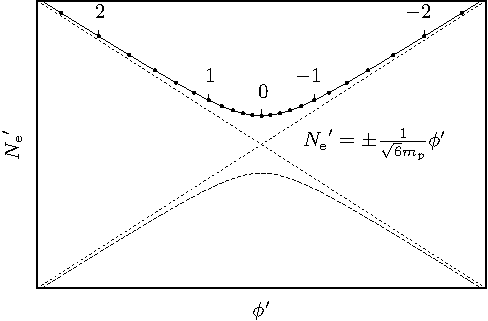
\includegraphics[width=\textwidth]{chapters/kinetic_dominance/figures/hyperbola}
  \caption{The constraint provided by the definition of $\Nflat$ in Halliwell time. The dynamical variables $\Nflatp$ and $\prm \phi$ lie on a hyperbola according to~\protect\eqref{eqn:Friedmann_tau}. A natural parametrization uses a hyperbolic angle $u$ detailed in~\protect\eqref{eqn:Ntrans} and~\protect\eqref{eqn:phitrans}. Note that only the upper half is parametrized, as the lower half of the hyperbola suggests a collapsing universe $(\Nflatp\propto H\propto\dot{a}<0)$. The points corresponding to $u\in\{-2,-1,0,1,2\}$ have been labeled to guide the eye.}\label{fig:figure_hyperbola}
\end{figure}
%
Applying the transformation above to the Halliwell-time evolution equations, we find that equation~\eqref{eqn:Friedmann_tau} is trivially satisfied, and equation~\eqref{eqn:Raychaudhuri_tau} takes the form:
%
\begin{equation}
  \frac{\Nflatp}{\prm{N}} \frac{\m}{\sqrt{6}}
  \left(\frac{\sqrt{2}}{\sinh u} \frac{\d{u}}{\d{\tau}} 
  - \frac{1}{\tanh u} \frac{\d{}}{\d{\phi}}\log V\right) 
  = -1.
  \label{eqn:master_tau}
\end{equation}
%

\subsection{Hamilton-Jacobi representation}
\label{sec:Hamilton-Jacobi_representations}
We reformulate the equation using the Hamilton-Jacobi representation; instead of considering the variables as functions of time $\tau$, one uses the field $\phi$ as the independent variable. Since we are considering universes with a monotonic inflaton $(\dot{\phi}\ne 0)$, the transformation from $t$ to $\phi$ is monotonic, and hence so too is that from $\tau$ to $\phi$.

One can switch to the Hamilton-Jacobi representation by changing the variables in the derivatives using the relation:
%
\begin{equation}
  \difrac{}{\tau}
  =
  \difrac{\phi}{\tau}\difrac{}{\phi}
  =
  \prm\phi\difrac{}{\phi}
  =
  -\sqrt{2}\sinh u \difrac{}{\phi},
  \label{eqn:tautrans}
\end{equation}
%
which on applying to equation~\eqref{eqn:master_tau} yields:
%
\begin{equation}
  \m\frac{\Nflatp}{\prm{N}} \sqrt{\frac{2}{3}}
  \left(\frac{\d{u}}{\d{\phi}} 
  + \frac{1}{2\tanh u} \frac{\d{}}{\d{\phi}}\log V\right) 
  = 
  1.
  \label{eqn:master_phi}
\end{equation}
%
We now  rescale the $\phi$ field into a new field $\psi$ via the relation:
%
\begin{equation}
  \frac{\d{}}{\d{\psi}} 
  = 
  \m\frac{\Nflatp}{\prm{N}}\sqrt{\frac{2}{3}}\frac{\d{}}{\d{\phi}}.
\end{equation}
%
More explicitly, $\psi$ is defined up to a constant by the monotonic transformation:
%
\begin{equation}
  \frac{\d{\psi}}{\d{\phi}} 
  = 
  \sqrt{\frac{3}{2}}\frac{\prm{N}}{\m\Nflatp} 
  \quad
  \Leftrightarrow\quad \psi 
  = 
  \sqrt{\frac{3}{2}}\frac{1}{\m}\int^\phi 
  \frac{\prm{N}}{\Nflatp}\:d\phi,
  \label{eqn:psi_by_phi}
\end{equation}
%
and this relationship is well defined since:
%
\begin{equation}
	\frac{\prm{N}}{\Nflatp} = \frac{H}{\Hflat} \ge 0.
\end{equation}
%
This rescaling absorbs all of the dependence on $\prm N$ and thus $\{\rho_i\}$ via~\eqref{eqn:N_H_relation} into the definition of $\psi$. Under the transformation~\eqref{eqn:psi_by_phi}, the master equation~\eqref{eqn:master_phi} takes the form:
%
\begin{equation}
  \frac{\d{u}}{\d{\psi}}  
  = 
  1-\frac{1}{\tanh u} \frac{\d{}}{\d{\psi}}\log \sqrt V.
\end{equation}
%
We have transformed the evolution equations~\eqref{eqn:Raychaudhuri_mod}--\eqref{eqn:Klein_Gordon_mod} into a single ``master equation'' in one variable, where all of the potential dependence is kept in a single term.

We may rearrange this slightly by making the monotonic transformation:
%
\begin{equation}
  u\mapsto y = \log\cosh(u), 
  \label{eqn:y_def}
\end{equation}
%
under which the master equation takes the form:
%
\begin{equation}
  \frac{\d{y}}{\d{\psi}} = \sqrt{1-e^{-2y}} - \frac{\d{}}{\d{\psi}}\log \sqrt V.
  \label{eqn:master_eq}
\end{equation}
%

\subsection{Interpreting the master equation}
\label{sec:interpreting_the_master_equation}

We now prove kinetic dominance by considering the asymptotics of the master equation~\eqref{eqn:master_eq} in the limit $a\rightarrow0$. We prove that there is at most a single solution $f(\psi)$ which is finite, with all of the rest diverging as $a\rightarrow0$. We finish by showing that a diverging solution $y(\psi)$ of the master equation is equivalent to kinetic dominance.

We begin by showing that $\psi$ diverges as $a\rightarrow0$. Through elementary derivative transformations with the chain rule and the definitions of various variables, we find:
%
\begin{align}
  \frac{\prm\phi}{\Nflatp} 
  &=
  \frac{\prm\psi\frac{\d{\phi}}{\d{\psi}}}{\Nflatp}
  &\text{(chain rule)} 
  \nonumber
  \\
  &=
  \m\sqrt{\frac{2}{3}}\frac{\prm\psi}{\prm{N}}  
  &\text{(from equation \protect\ref{eqn:psi_by_phi})} 
  \nonumber
  \\
  &=
  \m\sqrt{\frac{2}{3}}\frac{\dot\psi}{\dot{N}}  
  &\text{(chain rule)} 
  \nonumber
  \\
  &=
  \m\sqrt{\frac{2}{3}}\frac{\d{\psi}}{\d{\log a}}
  &\text{(since $H=\frac{\d{}}{\d{t}}\log a$)}.
  \label{eqn:div_psi}
\end{align}
%
From Figure~\ref{fig:figure_hyperbola} it is easy to see that:
%
\begin{equation}
  \left|\frac{\prm\phi}{\Nflatp}\right| > \sqrt{6}\m, 
\end{equation}
%
so combining this with equation~\eqref{eqn:div_psi} yields:
%
\begin{equation}
  \left|\frac{\d{\psi}}{\d{\log a}}\right| > 3. 
\end{equation}
%
From this is it easy to see that as $a\to0$, $\log a\to-\infty$ and so $|\psi|\to\infty$. The sign of the divergence of $\psi$ can be found by considering the monotonic transformations we have made: %
\begin{equation}
  t
  \xrightarrow{\protect\eqref{eqn:tau_def}}
  \tau
  \xrightarrow{\protect\eqref{eqn:phitrans}}
  \phi
  \xrightarrow{\protect\eqref{eqn:psi_by_phi}}
  \psi.
\end{equation}
%
By considering the equations denoted above, one can see that $\frac{\d{\tau}}{\d{t}}>0$, $\frac{\d{\psi}}{\d{\phi}}>0$, and $\frac{\d{\phi}}{\d{\tau}} = -\sqrt{2}\sinh u$. Thus as $a$ and $t$ decrease, one finds that if $u>0$, then $y>0$ by~\eqref{eqn:y_def} and thus $\psi\to\infty$.\footnote{This explains the choice of sign in the parametrization~\protect\eqref{eqn:phitrans}}



As we are considering universes where $\dot{\phi}\ne 0$, this places the constraint that:
%
\begin{equation}
  u 
  = 
  \sinh^{-1}\left(\frac{\prm\phi}{\sqrt 2}\right) 
  = 
  \sinh^{-1}\left(\frac{\dot\phi}{\sqrt 2 V(\phi)}\right)
  \ne 
  0,
\end{equation}
%
and by~\eqref{eqn:y_def}, we find that $y\ne0$ also.  The problem therefore breaks down into two cases: 
%
\begin{enumerate}
  \item $y>0$ and $\psi\rightarrow\infty$
  \item $y<0$ and $\psi\rightarrow -\infty$.
\end{enumerate}
%
We will consider the first case; the second may be treated in exactly the same way, with a couple of sign changes.  We now show that there is at most one {\em finite\/} solution $u$ satisfying the master equation~\eqref{eqn:master_eq} while remaining positive ($u>0$).

Let us assume that there exists a solution $f(\psi)$ of~\eqref{eqn:master_eq} that is positive and finite ($0<f<\fm$ for some finite $\fm$):
%
\begin{equation}
  \difrac{f}{\psi} = \sqrt{1-e^{-2f}} -\frac{\d{}}{\d{\psi}}\log \sqrt V.
  \label{eqn:master_eq_f}
\end{equation}
%
where:
%
\begin{equation}
  0<f(\psi)<\fm,
\end{equation}
%
and assume some initial condition on $f$ at some finite value
$\psi=\psiz$:
%
\begin{equation}
  f(\psiz)=\fz.
\end{equation}
%
Now consider a solution $h(\psi)$ with some larger initial value:
%
\begin{equation}
  h(\psiz)=\hz>\fz.
\end{equation}
%
Since $h$ is also a solution of the master equation~\eqref{eqn:master_eq} it satisfies:
%
\begin{equation}
  \difrac{h}{\psi} = \sqrt{1-e^{-2h}} -\frac{\d{}}{\d{\psi}}\log \sqrt V.
  \label{eqn:master_eq_h}
\end{equation}
%
Taking the difference of~\eqref{eqn:master_eq_f} and~\eqref{eqn:master_eq_h} gives:
%
\begin{equation}
  \frac{\d{}}{\d{\psi}}\left(h-f\right)
  = 
  \sqrt{1-e^{-2h}}-\sqrt{1-e^{-2f}}
  \label{eqn:master_eq_diff}
\end{equation}
%
By a uniqueness theorem, discussed in Section~\ref{sec:uniqueness_theorem}, if $h(\psiz)>f(\psiz)$, then $h(\psi_1)>f(\psi_1)$ (for $\psi_1\ne\psi_0$). Therefore one can see from~\eqref{eqn:master_eq_diff} that the difference between $h$ and $f$ is monotonically increasing in any finite interval $[\psiz,\psi_1]$.  One can thus conclude that:
%
\begin{equation}
  h-f>\hz-\fz=\Delta_0>0
  \label{eqn:cosh_rel}
\end{equation}
%
where we have defined $\Delta_0 = \hz-\fz$, and $h$ and $f$ are evaluated at the end of the interval $\psi_1$. Since $h>\Delta_0+f$, it is easy to see using~\eqref{eqn:master_eq_diff} that:
%
\begin{equation}
  \frac{\d{}}{\d{\psi}}\left(h-f\right)
  > 
  \sqrt{1-e^{-2(f+\Delta_0)}}-\sqrt{1-e^{-2f}}
\end{equation}
%
This is a monotonically decreasing function of $f$, and hence attains its minimum at $\fm$; thus,
%
\begin{equation}
  \frac{\d{}}{\d{\psi}}\left(h-f\right)
  > 
  \sqrt{1-e^{-2(\fm+\Delta_0)}}-\sqrt{1-e^{-2\fm}} 
  >
  0.
\end{equation}
%
The difference between $h$ and $f$ is therefore monotonically increasing at a rate greater than some positive number. Since $f$ is positive, it is bounded below and as $\psi_1$ is made arbitrarily large, $h$ grows without bound.

%
\begin{figure}[tp]
  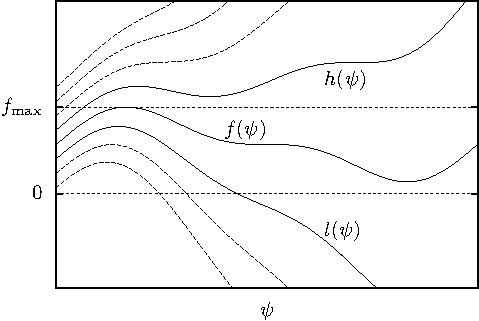
\includegraphics[width=\textwidth]{chapters/kinetic_dominance/figures/uschem}
  \caption{In general there is at most a single solution $f(\psi)$ to the master equation~\protect\eqref{eqn:master_eq} that is positive and finite $0<f(\psi)<\fm$. Any solution $h(\psi)$ that begins higher than $f(\psi)$ must diverge. Consequently, any solution $l(\psi)$ that begins lower than $f(\psi)$ cannot remain above $0$. If it were able to, then $l(\psi)$ would also be another finite solution lying between $0$ and some $l_\smax$. By the previous argument, this would mean $f$ could not be finite, contradicting our initial assumption.\label{fig:figure_uschem}}
\end{figure}
%
We therefore find ourselves in a situation demonstrated in Figure~\ref{fig:figure_uschem}. For any given potential $V(\phi)$, there is at most a single solution $f(\psi)$ that is finite and positive [$0<f(\psi)<\fm$]: any solution that is larger than $f(\psi)$ at some point $\psi=\psiz$ diverges as $\psi\to\infty$ ($a\to0$). Further, any solution $l(\psi)$ that starts out less than $f(\psi)$ must fall to a value less than $0$.  If $l(\psi)$ did not fall below $0$, but were another example of a finite positive solution, then by the argument above, this would imply $f(\psi)>l(\psi)$ must diverge, contradicting our initial assumptions on $f(\psi)$.

One therefore expects universes with a steadily moving inflaton to have a generically diverging $y$ as $a\to0$, except perhaps for a single special case for a given potential $V(\phi)$.  The consequences of a generically divergent $y$ shall now be examined.  If $y$ diverges, then so does $u$ by equation~\eqref{eqn:y_def}. If $u$ diverges, then we find that $\prm \phi$ diverges by~\eqref{eqn:phitrans}:
%
\begin{equation}
  \frac{\d{\phi}}{\d{\tau}}=\prm{\phi} 
  = 
  -\sqrt{2}\sinh u\rightarrow -\infty.
\end{equation}
%
Converting back from Halliwell time to cosmic time using equation~\eqref{eqn:tau_def} shows:
%
\begin{equation}
  \prm{\phi}^2 
  = 
  \frac{\dot{\phi}^2}{V(\phi)}
\end{equation}
%
One can thus see that the divergence of $y$, $u$ and $\prm \phi$ therefore requires that:
%
\begin{equation}
  \lim\limits_{y\to\pm\infty} \frac{\dot\phi^2}{V(\phi)}
  =
  \lim\limits_{a\to 0} \frac{\dot\phi^2}{V(\phi)} = \infty,
  \label{eqn:kdfinal}
\end{equation}
%
which is equivalent to saying that $\dot{\phi}^2\gg V(\phi)$ as
$a\to0$. The early Universe is generically kinetically dominated.

\section{Consequences of kinetic dominance}
\label{sec:consequences_of_kinetic_dominance}

The condition $\dot\phi^2\gg V(\phi)$ for kinetic dominance allows one to derive several results. First, the kinetic energy of the inflaton dominates over the other fluids as $a\to 0$, allowing us at early times to neglect any additional effects such as curvature, radiation, matter or a cosmological constant. Second, the Universe emerges from an initial singularity at a finite co\"{o}rdinate time, which may be taken as $t=0$. Finally, one is able to determine exact analytic expressions for the solutions in co\"{o}rdinate or conformal time for each of the cases where curvature, radiation, matter or a cosmological constant are present.


\subsection{Dominance of $\dot{\phi}^2$ over other fluids}
\label{sec:dominance_fluids}
In the limit that $a\to 0$, the auxiliary fluid with the largest value of $w$ dominates over all of the others. Along with kinetic dominance, we can therefore assume that the Raychaudhuri~\eqref{eqn:Raychaudhuri_mod} and Friedmann~\eqref{eqn:Friedmann_mod} equations take the form:
%
\begin{align}
  \dot{H}+H^2 
  &= 
  -\frac{\dot{\phi}^2}{3\m^2} - \frac{1}{6\m^2}(1+3w)\rho_w
  \label{eqn:Ray_KD_eq_rho}
  \\
  H^2 
  &= 
  \frac{\dot{\phi}^2}{6\m^2} +  \frac{1}{3\m^2}\rho_w,
  \label{eqn:Friedmann_KD_eq_rho}
\end{align}
  %
where $\rho_w$ is the density of the auxiliary fluid with the largest $w$.  It is not difficult to show using equation~\eqref{eqn:rho_a},
along with $H=\frac{\d{}}{\d{t}}\log a$ that these equations solve to give:
%
\begin{align}
  H^2 
  &= 
  \frac{1}{3\m^2}\left(\frac{\beta^2}{a^6} + \rho_w\right) 
  \label{eqn:H_of_a_1}
  \\
  \dot{\phi}^2 
  &= 
  2\frac{\beta^2}{a^6} 
  \label{eqn:dotphi_of_a_1}
\end{align}
%
where $\beta$ is an integration constant. From this, if $w<1$ then as
$a\to 0$, one finds:
%
\begin{equation}
  \dot{\phi}^2 \propto a^{-6} 
  \gg
  \rho_w \propto a^{-3(1+w)}.
  \label{eqn:dotphidom}
\end{equation}
%
Thus, the kinetic term of the inflaton dominates over all other fluids with $w<1$.




Historically, inflationary potentials were considered in the context of grand unified theories \citep{PhysRevLett.48.1220,linde_1982} which resulted in an effective potential $V(\phi,T)$ depending on the value of the field $\phi$ and a temperature.  This was then developed \citep{1995PhRvL..74.1912B,PhysRevLett.75.3218} into a theory in which the inflaton remains in thermal equilibrium with an auxiliary radiation fluid.

More recent work \citep{2007PhRvD..76f3512P} typically assumes that the inflaton is decoupled from the auxiliary fluids in the preinflationary phase, and that the Universe is {\em radiation dominated\/} at this early stage. Given the above result~\eqref{eqn:dotphidom}, such assumptions may now need revisiting.



\subsection{Finite time singularity}

Since $H = \dot{a}/a$, we can express the co\"{o}rdinate time $t$ as an integral: 
%
\begin{equation}
  t = \int \frac{\d{a}}{aH}.
\end{equation}
%
From equation~\eqref{eqn:H_of_a_1}, one can see that ${(aH)}^{-1}$ is finite as $a\to0$. By the above integral, this shows that the Universe emerges at a finite time in the past, which can be taken as $t=0$.  Moreover, from~\eqref{eqn:dotphidom}, the (dominant) energy density of the Universe scales as $a^{-6}$ as $a \to 0$, showing that $t=0$ is a singularity.

\subsection{Analytic solutions for the kinetically dominated universe} 
If one considers the solutions of the Raychaudhuri and Friedmann equations~\eqref{eqn:Raychaudhuri_mod} and~\eqref{eqn:Friedmann_mod} in the limit that $a\to0$, then one can neglect the potential term $V(\phi)$ as it is suppressed by $\dot{\phi}^2$. In addition, the other fluid terms are negligible in comparison to the term with the largest $w$.  When these considerations are taken into account, the evolution equations take the form shown in~\eqref{eqn:Ray_KD_eq_rho} and~\eqref{eqn:Friedmann_KD_eq_rho}. One can find solutions for $\phi(a),H(a)$ and $\rho_w(a)$ parametrically in terms of $a$.  In addition, one can find co\"{o}rdinate time $t(a)$ in terms of $a$ using the relation:
%
\begin{equation}
  t = \int \frac{\d{a}}{aH(a)}.
\end{equation}
%
Conformal time $\eta$ is defined by the equation $\dot{\eta} =
a^{-1}$, and can be found in terms of $a$ using:
%
\begin{equation}
  \eta = \int \frac{\d{a}}{a^2H(a)}.
\end{equation}
%
The solutions are:
%
\begin{align}
  \rho_w(a) 
  &\propto 
  a^{-3(1+w)} 
  \\
  H{(a)}^2 
  &= 
  \frac{1}{3\m^2}\left(\frac{\beta^2}{a^6} + \rho_w\right)  
  \label{eqn:H_of_a}
  \\
  \dot{\phi}{(a)}^2
  &=
  2\frac{\beta^2}{a^6} 
  \label{eqn:dotphi_of_a}
  \\
  \phi(a)
  &=
  c + \pm
  \sqrt{\frac{2}{3}}\frac{\m}{1-w} \ln \left[ 
  \frac 
  {{a}^{3(1-w)}}
  {{\left(\sqrt{1+\frac{\rho_w{a}^{6}}{\beta^2}}+1\right)}^2} 
  \right]  
  \label{eqn:phi_of_a}
  \\
  t(a)
  &=
  a^3 \frac{\m\sqrt{3}}{3\beta} 
  \:\: 
  {_2F_1}(
  \frac{1}{2},
  \frac{1}{1-w};
  \frac{2-w}{1-w},
  -\frac{a^6\rho_w}{\beta^2}
  ) 
  \label{eqn:t_of_a}
  \\
  \eta(a) 
  &= 
  a^2 \frac{\m\sqrt{3}}{2\beta}
  \:\: 
  {_2F_1}(
  \frac{1}{2},
  \frac{2}{3(1-w)};
  \frac{5-3w}{3(1-w)},
  -\frac{a^6\rho_w}{\beta^2}
  ),
  \label{eqn:eta_of_a}
\end{align}
%
where $\beta$ and $c$ are constants of integration which will be redefined shortly. We have chosen $t,\eta$ such that $a\to0$ as $t,\eta \to 0$.


For specific values of $w$, the hypergeometric functions $_2F_1$ take simple forms. If $w=-1$ or $0$, then equation~\eqref{eqn:t_of_a} is expressible in closed form, in terms of trigonometric and algebraic functions in $a$ respectively. If $w=-1/3$ or $1/3$, then~\eqref{eqn:eta_of_a} may be expressed in closed form. In each of these cases, these equations are invertible giving an expression for $a(t)$ or $a(\eta)$.  We note that, except for the case $w=-1/3$, the solutions~\eqref{eqn:H_of_a}--\eqref{eqn:eta_of_a} correspond to a spatially flat universe.

We shall examine each of the above cases in turn, after first looking at the case in which there are no auxiliary fields, $\rho_w=0$.  In so doing, it will prove useful to define the functions:
%
\begin{equation}
  \begin{array}{rr}
    S_k(x),&S_k^{-1}(x)
    \\ 
    C_k(x),&C_k^{-1}(x)
    \\ 
    T_k(x),&T_k^{-1}(x)
    \\
  \end{array}
  =
  \left\{
%
  \begin{array}{rl}
%
    \begin{array}{rr}
      \sin(x),&\arcsin(x)
      \\ 
      \cos(x),&\arccos(x)
      \\ 
      \tan(x),&\arctan(x)
      \\
    \end{array}
%
    &: k>0 \\
%
    \begin{array}{rr}
      x,&x
      \\ 
      1,&1
      \\ 
      x,&x
      \\
    \end{array}
%
    &: k=0 \\
%
    \begin{array}{rr}
      \sinh(x),&\arcsinh(x)
      \\ 
      \cosh(x),&\arccosh(x)
      \\ 
      \tanh(x),&\arctanh(x)
      \\
    \end{array}
%
    &: k<0
  \end{array}
%
  \right. 
\end{equation}
%

\subsubsection{No auxiliary fields, $\rho_w=0$}
If $\rho_w=0$, then equation~\eqref{eqn:t_of_a} becomes:
%
\begin{equation}
  t = a^3 \frac{\m\sqrt{3}}{3\beta}.
\end{equation}
%
One can rearrange this to find $a$ as a function of $t$,
%
\begin{equation}
  a(t)
  =
  t^{1/3} {\left(\frac{3\beta}{\m\sqrt{3}}\right)}^{1/3},
  \label{eqn:a_of_t_beta_flat}
\end{equation}
%
and then substitute this into equations~\eqref{eqn:H_of_a} and~\eqref{eqn:dotphi_of_a} to find:
%
\begin{align}
  H(t) 
  &= 
  \frac{1}{3t}, 
  \label{eqn:H_of_t_flat} 
  \\
  \dot{\phi}(t) 
  &= 
  \pm\sqrt{\frac{2}{3}}\frac{\m}{t}.
  \label{eqn:dotphi_of_t_flat}
\end{align}
%
The latter integrates to give:
%
\begin{equation}
  \phi(t) 
  = 
  \phip \pm\sqrt{\frac{2}{3}}\m\log\left(\frac{t}{\tp}\right),  
  \label{eqn:phi_of_t_flat}
\end{equation}
%
where $\phip$ is an integration constant chosen such that $\phi(\tp)=\phip$, where $\tp$ is some time. It is more appropriate to redefine the integration constant $\beta$ as:
%
\begin{equation}
  \beta 
  \equiv 
  \frac{\Rp^3\m}{\tp\sqrt{3}}, 
  \label{eqn:beta_def}
\end{equation}
%
since then, equation~\eqref{eqn:a_of_t_beta_flat} for $a(t)$ becomes:
%
\begin{equation}
  a(t) 
  = 
  \Rp {\left(\frac{t}{\tp}\right)}^{1/3},
  \label{eqn:a_of_t_flat}
\end{equation}
%
which is more in keeping with equation~\eqref{eqn:phi_of_t_flat}.  

For this case, one can also obtain analytical solutions in terms of conformal time.  If $\rho_w=0$ and $\beta$ is defined by~\eqref{eqn:beta_def}, equation~\eqref{eqn:eta_of_a} becomes:
%
\begin{equation}
  \eta(t) 
  = 
  a^2 \frac{\m\sqrt{3}}{2\beta}
  =
  \frac{3\tp}{2\Rp^3}a^2.
  \label{eqn:eta_of_t}
\end{equation}
%
Using equation~\eqref{eqn:a_of_t_flat}, we can show:
%
\begin{equation}
  \eta
  =
  \etap{\left(\frac{t}{\tp}\right)}^{2/3},
\end{equation}
%
where we have defined $\etap$ as:
%
\begin{equation}
  \etap
  =
  \frac{3\tp}{2\Rp}.
  \label{eqn:etap_eq}
\end{equation}
%
Now we have $\eta(t)$ in equation~\eqref{eqn:eta_of_t}, we can change equations~\eqref{eqn:H_of_t_flat},~\eqref{eqn:dotphi_of_t_flat},~\eqref{eqn:phi_of_t_flat} and~\eqref{eqn:a_of_t_flat} to:
%
\begin{align}
  a(\eta)
  &=
  \Rp {\left(\frac{\eta}{\etap}\right)}^{1/2},
  \\
  H(\eta)
  &=
  \frac{1}{3\tp}{\left(\frac{\eta}{\etap}\right)}^{-3/2},
  \\
  \dot{\phi}(\eta)
  &=
  \pm\sqrt{\frac{2}{3}}
  \frac{\m}{\tp}{\left(\frac{\eta}{\etap}\right)}^{-3/2},
  \\
  \phi(\eta)
  &=
  \phip \pm\sqrt{\frac{3}{2}}\m\log\left(\frac{\eta}{\etap}\right). 
  \label{eqn:phi_flat}
\end{align}
%

It should be noted that since $\dot{\phi}^2 \gg \rho_w$ at sufficiently early times, all solutions reduce to the above forms for small enough $t$ or $\eta$. We can thus fix the form of solutions with nonzero $\rho_w$ by matching onto the above solutions for sufficiently small $t$ or $\eta$.  

\subsubsection{Dark energy, $w=-1$}
For dark energy in the form of a cosmological constant, we find that the energy density in standard notation is:
%
\begin{equation}
  \rho_w = \m^2\Lambda.
\end{equation}
%
For $w=-1$, equation~\eqref{eqn:t_of_a} is expressible in terms of trigonometric functions, and may be rearranged to express the scale factor $a$ in terms of co\"{o}rdinate time. Once $a(t)$ is obtained, the remaining equations~\eqref{eqn:H_of_a},~\eqref{eqn:dotphi_of_a} and~\eqref{eqn:phi_of_a} can be used to express the rest of the variables in terms of $t$. Using our definition of $\beta$ [equation \nolinebreak\ref{eqn:beta_def}], and defining the new time scale,
%
\begin{equation}
  \tL = \frac{1}{\sqrt{3\Lambda}},
  \label{eqn:tl}
\end{equation}
%
the solutions are:
%
\begin{align}
  a(t)
  &=
  \Rp{\left[{\frac {S_{-\Lambda}(t/\tL)}{\tp/\tL}}\right]}^{1/3},
  \\
  H(t)
  &=
  \frac{1}{3\tL}\frac{1}{T_{-\Lambda}(t/\tL)},
  \\
  \dot{\phi}(t)
  &=
  \sqrt{\frac{2}{3}}\frac{\m}{\tL}\frac{1}{S_{-\Lambda}(t/\tL)},
  \\
  \phi(t)
  &=
  \phip \pm \sqrt{\frac{2}{3}}\m
  \log\left[
  \frac{\tL}{\tp} 
  \frac 
  {2\: S_{-\Lambda} \left( t/\tL \right) }
  {1 + C_{-\Lambda} \left( t/\tL \right)}  
  \right].
\end{align}
%

\subsubsection{Spatial curvature, $w=-1/3$}
Spatial curvature is equivalent to a fluid with equation-of-state parameter $w=-1/3$ and density:
%
\begin{equation}
  \rho_w = -3\m^2\frac{\kappa}{a^{2}}.
\end{equation}
%
For $w=-1/3$, equation~\eqref{eqn:eta_of_a} is expressible in terms of trigonometric functions, and may be rearranged to express the scale factor $a$ in terms of conformal time. Once $a(\eta)$ is obtained, the remaining equations~\eqref{eqn:H_of_a},~\eqref{eqn:dotphi_of_a} and~\eqref{eqn:phi_of_a} can be used to express the rest of the variables in terms of $\eta$. Using our definitions of $\beta$ [equation \nolinebreak\ref{eqn:beta_def}] and $\etap$ [equation \nolinebreak\ref{eqn:etap_eq}], and defining the new time scale,
%
\begin{equation}
  \etak = \frac{1}{2\sqrt{\kappa}},
  \label{eqn:etak}
\end{equation}
%
the solutions are:
%
\begin{align}
  a(\eta)
  &=
  \Rp{\left[
  \frac
  {S_\kappa\left(\eta/\etak\right)}
  {\etap/\etak} \right]}^{1/2},
  \\
  H(\eta)
  &=
  \frac{1}{3\tp}
  \frac{{(\etap/\etak)}^{3/2}}
  {T_\kappa(\eta/\etak)\sqrt{S_\kappa(\eta/\etak)}}, 
  \\
  \dot{\phi}(\eta)
  &=
  \pm\sqrt{\frac{2}{3}}
  \frac{\m}{\tp}
  {\left[
  \frac
  {\etap/\etak}
  {S_{\kappa}(\eta/\etak)}
  \right]}^{3/2},
  \\
  \phi(\eta) 
  &=
  \phip \pm \sqrt{\frac{3}{2}}\m\log  \left[
  \frac{\etak}{\etap} 
  \frac{2\:S_{\kappa}\left(\eta/\etak \right) }
  {1 + C_{\kappa} \left( \eta/\etak \right)   }  
  \right]. 
\end{align}
%



\subsubsection{Matter, $w=0$}
For matter with zero pressure, one has $w=0$ and so:
%
\begin{equation}
  \rho_w = \rhomp{\left(\frac{a}{\Rp}\right)}^{-3},
\end{equation}
%
where $\rhomp$ is an integration constant, labeling the energy density of matter at the epoch $\Rp$.  For $w=0$, equation~\eqref{eqn:t_of_a} is expressible as an algebraic function, and may be rearranged to express the scale factor $a$ in terms of co\"{o}rdinate time. Once $a(t)$ is obtained, the remaining equations~\eqref{eqn:H_of_a},~\eqref{eqn:dotphi_of_a}~\&~\eqref{eqn:phi_of_a} can be used to express the rest of the variables in terms of $t$. Using our definition of $\beta$ (equation~\ref{eqn:beta_def}), and defining the new time scale,
%
\begin{equation}
  \tm = \frac{4\m^2}{3\tp\rhomp },
  \label{eqn:tm}
\end{equation}
%.
the solutions are:
%
\begin{align}
  a(t)
  &=
  \Rp{\left(\frac{t}{\tp}\right)}^{1/3}
  {\left(1+\frac{t}{\tm}\right)}^{1/3} ,
  \\
  H(t) &= 
  \frac{1+2\frac{t}{\tm}}{3t{{\left( 1+\frac{t}{\tm} \right) }}},
  \\
  \dot{\phi}(t) &= 
  \pm\sqrt{\frac{2}{3}}\m
  \frac{1}
  {t \left( 1+\frac{t}{\tm} \right) },
  \\
  \phi(t) &=
  \phip \pm \sqrt{\frac{2}{3}}\m \log\left[  
  \left(\frac{t}{\tp}\right) 
  \frac {1}{1+\frac{t}{\tm}}  
  \right].
\end{align}
%




\subsubsection{Radiation, $w=1/3$}

For radiation one has $w=1/3$, and so:
%
\begin{equation}
  \rho_w = \rhorp{\left(\frac{a}{\Rp}\right)}^{-4},
\end{equation}
%
where $\rhorp$ is an integration constant, labeling the energy density of matter at the epoch $\Rp$.  For $w=1/3$, equation~\eqref{eqn:eta_of_a} is expressible as an algebraic function, and may be rearranged to express the scale factor $a$ in terms of co\"{o}rdinate time. Once $a(\eta)$ is obtained, the remaining equations~\eqref{eqn:H_of_a},~\eqref{eqn:dotphi_of_a} and~\eqref{eqn:phi_of_a} can be used to express the rest of the variables in terms of $\eta$. Using our definition of $\beta$~\ref{eqn:beta_def}, and $\etap$~\ref{eqn:etap_eq}, and defining the new time scale,
%
\begin{equation}
  \etar = \frac{3\m^2}{\Rp^2\etap\rhomp}.
  \label{eqn:etar}
\end{equation}
%
the solutions are:
%
\begin{align}
  a(\eta)
  &=
  \Rp{\left(\frac{\eta}{\etap}\right)}^{1/2}
  {\left({1+\frac{\eta}{\etar}}\right)}^{1/2},
  \\
  H(\eta) 
  &= 
  \frac{1}{3\tp}{\left(\frac{\eta}{\etap}\right)}^{-3/2}
  \frac{1+ 2\frac{\eta}{\etar}}
  {{\left(1+ \frac{\eta}{\etar}\right)}^{3/2}},
  \\
  \dot{\phi}(\eta) 
  &=
  \sqrt{\frac{2}{3}}\frac{\m}{\tp}
  {\left(\frac{\eta}{\etap}\right)}^{-3/2}
  \frac{1}{{\left(1+ \frac{\eta}{\etar}\right)}^{3/2}},
  \\ 
  \phi(\eta) 
  &=
  \phip+\sqrt {\frac{3}{2}}\m\log  
  \left[
  \left(\frac{\eta}{\etap}\right)
  \frac {1}{\left(1+ \frac{\eta}{\etar}\right)} 
  \right] 
\end{align}
%

\subsection{The constants of integration}
\label{sec:constants}
In the previous section, several constants arose, which we shall now review. For the system of equations~\eqref{eqn:Ray_KD_eq_rho}--\eqref{eqn:Friedmann_KD_eq_rho}, one would expect four constants of integration. The first is chosen by setting $a=0$ at $t=0$. For the case $\rho_w=0$, the second and third are chosen by choosing a later time $\tp>0$ and fixing:
%
\begin{align}
  \phi(\tp) &= \phip, \nonumber\\
  a(\tp) &= \Rp. \nonumber
\end{align}
%
We can also determine conformal time in this case, which involved defining a new constant $\etap$ in terms of $\Rp$ and $\phip$ via equation~\eqref{eqn:etap_eq}, and the solutions may be determined in conformal time. For the remaining cases, there is an additional integration constant determined by the value of $\rho_w$ when the scale factor is $\Rp$. The solutions for these cases are then determined by matching them onto the case $\rho_w=0$ at early times.

In addition, we defined a relevant time scale for each of the $\rho_w \neq 0$ cases: $\tL$, $\etak$, $\tm$, $\etar$. These are expressed in terms of the previous integration constants in equations~\eqref{eqn:tl},~\eqref{eqn:etak},~\eqref{eqn:tm} and~\eqref{eqn:etar}. If one chooses $\tp$ or $\etap$ to be much less than this second time scale, then the Universe is in a fully kinetically dominated regime at $\tp$, $\etap$, with solutions very close to the $\rho_w=0$ case. When $\eta$ is of the order of the second time scale, then the effects of the Universe's (dominant) additional component can be seen.

Although we have determined these equations in terms of three integration constants, there are in fact only two.  The evolution equations~\eqref{eqn:Raychaudhuri_mod}~\&~\eqref{eqn:Friedmann_mod} possess a two-parameter symmetry corresponding to a rescaling of $a$ and $t$. More precisely, the form of the equations does not change under the transformation:
%
\begin{equation}
  a\mapsto\alpha a, 
  \qquad 
  t \mapsto\sigma^{-1}t,
\end{equation}
%
provided that $\rho_i$ and the potential transform as:
%
\begin{equation}
  \rho_i \mapsto \alpha^{3(1+w_i)}\sigma^2\rho_i, 
  \qquad
  V(\phi) \mapsto \sigma^2 V(\phi)
\end{equation}
%
This symmetry can be used effectively to remove some of the remaining integration constants. In practice this means that one may set $\tp=1$ to be the Planck time and the scale factor $a(\tp)=\Rp=1$. Usually one takes the scale factor to be unity at the present epoch $a_0\equiv a(t_0)=1$, but this requirement is complicated by the uncertainties of reheating, so we do not follow that convention here. One may ``physically'' interpret $\phip$ as the value of the field at $t=t_p$.  This requires extrapolating the classical equations far beyond their validity, so it is more of a mnemonic aid than a physical interpretation.  As we will see below, $\phip$ controls the total number of $e$-folds of inflation.













\section{Kinetic dominance in action}
\label{sec:Kinetic_dominance_in_action}

We shall now demonstrate the utility of kinetic initial conditions in the analysis of inflationary models. Even without integrating the evolution equations for $H(t)$ and $\phi(t)$, one sees that the basic scenario entails the Universe emerging from an initial singularity at $t=0$ in a regime where the kinetic energy of the inflaton dominates its potential energy along with any curvature or additional fluids.  The evolution of $H(t)$ and $\phi(t)$ in this regime are given by~\eqref{eqn:H_of_t_flat} and~\eqref{eqn:phi_of_t_flat} at sufficiently early times.  $H(t)$ and $|\phi(t)|$ and their time derivatives decrease during this period of kinetic dominance, which concludes when there is approximate equipartition $\dot{\phi}^2 \sim V(\phi)$ between the kinetic and potential energies of the inflaton.  This marks the onset of a (typically brief) period of fast-roll inflation \citep{Linde:2001}, which must eventually become slow-roll inflation, with $\dot{\phi}^2 \ll V(\phi)$, since the latter is a generic attractor solution for inflation models \citep{belinsky_inflationary_1985}.  We will see that integration of the equations of motion in some illustrative cases does indeed verify these expectations.

For simplicity we shall work in the case with no other additional fields, $\rho_w=0$, although our methods apply equally well to more complicated solutions. After discussing the validity of the initial conditions and numerical techniques, we shall consider two forms of potential: polynomial and exponential.

\subsection{Initial conditions and scaling}

For $\rho_w=0$ the Universe is spatially flat and contains only the inflaton field. The evolution equations then take the form:
%
\begin{align}
  H^2 
  &= 
  \frac{1}{3\m^2}
  \left(\frac{1}{2}\dot{\phi}^2 + V(\phi) + \sum_i\rho_i\right),
  \label{eqn:Friedmann_eq} 
  \\
  0
  &= 
  \ddot{\phi} +3\dot{\phi}^2H + V^\prime(\phi).
  \label{eqn:Motion_eq_Scalar}
\end{align}
%
The general solution to the evolution equations has the asymptotic form given in equations~\eqref{eqn:H_of_t_flat} and~\eqref{eqn:phi_of_t_flat}. As discussed in Section~\ref{sec:constants}, we may choose $\tp=1$ to be the Planck time. Given this, we set the initial conditions at an initial time $\ti$ as:
%
\begin{align}
  \phi(\ti) \equiv \phii
  &= 
  \phip - \sqrt{\frac{2}{3}}\m\log \ti, 
  \label{eqn:phi_ic}
  \\
  \dot\phi(\ti) 
  \equiv 
  \phidi
  &= 
  -\sqrt{\frac{2}{3}}\frac{\m}{\ti}, 
  \label{eqn:phid_ic}
  \\
  H(\ti) 
  \equiv 
  \Hi
  &= 
  \frac{1}{3\ti}. 
  \label{eqn:H_ic}
\end{align}
There is a single constant of integration $\phip$, which directly controls the number of $e$-folds during inflation. The number of $e$-folds $N_*$ between the pivot scale $k_*$ and the end of inflation is typically $50$--$60$ \citep{planck_collaboration_planck_2013-1}. For the rest of this paper $\phip$ will be chosen so that the total number of $e$-folds $N_\mathrm{tot}=55$. This will be discussed in greater detail in Section~\ref{sec:powspec}.

Throughout this paper we work in the classical regime. In order for the conditions above to be valid, the initial conditions must be set at a time greater than the Planck time, $\ti >\tp=1$, but within the kinetic dominated regime, for which $V(\phii) \ll \phidi^2$. Setting $\ti=\tp=1$ in the above, one sees that kinetic dominance will endure beyond the Planck time provided:
%
\begin{equation}
  V(\phip) \ll \m^2.
\end{equation}
%
The above requirement typically holds for potentials that give physically reasonable inflation models. For example, in the case of a free inflaton with mass $m$, one has \[ V(\phi) = \frac{1}{2}m^2 \phi^2.\] In order to generate the correct amplitude of curvature perturbations, the mass must be of the order $m\sim10^{-5}\m$, whereas to generate the correct number of $e$-folds one requires $\phip\bigO{10}$, in which case $V(\phip) \sim 10^{-8} \m^2$.  Thus, there is no need to advocate trans-Planckian physics, since kinetic dominance lasts well beyond the Planck time, so one can set $\ti \gg \tp$.


We note that the evolution equations~\eqref{eqn:Friedmann_eq}~\&~\eqref{eqn:Motion_eq_Scalar} are invariant under  the simultaneous rescaling of the time co\"{o}rdinate, Hubble parameter and inflaton potential:
%
\begin{align}
  t 
  &\longmapsto 
  \sigma^{-1}t,
  \\
  H 
  &\longmapsto 
  \sigma H,
  \\
  V(\phi) 
  &\longmapsto
  \sigma^2 V(\phi).
\end{align}
%
The advantage of this for numerical work is that a multiplicative scaling parameter from the potentials can be removed without loss of generality.


\subsection{Polynomial potentials}
\label{sec:section_polynomial_potentials}
We begin by analyzing examples of polynomial potentials of the form:
%
\begin{equation}
  \Vpol(\phi) = \mu^2\phi^n.
  \label{eqn:polpot}
\end{equation}
%
To obtain results we integrate the evolution equations~\eqref{eqn:Friedmann_eq}~\&~\eqref{eqn:Motion_eq_Scalar} numerically.  Our kinetic initial conditions are chosen using equation~\eqref{eqn:phi_ic}--\eqref{eqn:H_ic} with an initial time $\ti$ small enough such that the inflaton is in the kinetic regime $V(\phii)\ll\dot{\phii}^2$. For the purposes of numerics the scaling parameter $\mu$ can be removed by rescaling the time co\"{o}rdinate (setting $\sigma=\mu^{-1}$). $\phip$ is set by requiring that there be $55$ $e$-folds during inflation.

%
\begin{figure}[tp]
  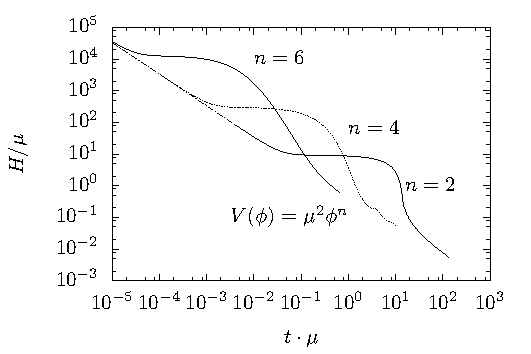
\includegraphics[width=\textwidth]{chapters/kinetic_dominance/figures/Hpol}
  \caption{The evolution of the Hubble parameter for three polynomial potentials of the form in~\eqref{eqn:polpot}. The axes have been rescaled in terms of the parameter $\mu$ in the potential, so that this graph describes the evolution for any choice of $\mu$. The initial conditions for inflation were set using the flat-universe kinetic conditions, and the parameter $\phip$ was chosen so as to give $55$ $e$-folds of inflation. All three universes emerge in a kinetically dominated phase with $H=1/(3t)$, before entering a slow-roll inflationary phase with $H\sim\mathrm{constant}$. The universe then exits inflation, after which small `wiggles' in $H$ can be seen. These are due to the field $\phi$ executing oscillations about the base of the potential.\label{fig:figure_Hpol}}
\end{figure}
%

%
\begin{figure}[tp]
  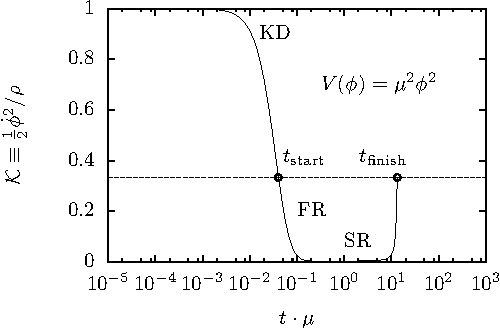
\includegraphics[width=\textwidth]{chapters/kinetic_dominance/figures/Kpol} 
  \caption{The evolution of $\Kfrac = \frac{1}{2}\dot{\phi}^2/\rho$ for the quadratic inflaton potential $V(\phi) = \mu^2 \phi^2$.  The Universe can be seen to begin in a kinetically dominated state (KD).  It enters inflation at $t_\mathrm{start}$. There is a brief fast-roll (FR) phase of inflation, before the Universe enters a protracted slow-roll (SR) phase. The Universe exits inflation at time $t_\mathrm{finish}$ after $55$ $e$-folds. After the end of inflation the field $\phi$ executes oscillations about the base of the potential. This causes $\Kfrac$ to oscillate rapidly between $0$ and $1$. For clarity, the value of $\Kfrac(t)$ with $t>t_\mathrm{finish}$ has not been plotted. The above behavior is common to all of the  polynomial potentials shown in Figure~\protect\ref{fig:figure_Hpol}.\label{fig:figure_Kpol}  }
\end{figure}
%

The evolution of the Hubble parameter is shown in Figure~\ref{fig:figure_Hpol} for polynomials with $n=2,4,6$. It is helpful to define the variable:
%
\begin{equation}
  \Kfrac 
  \equiv  
  \frac{\frac{1}{2}\dot{\phi}^2  }{\rho}  
  =  
  \frac{\frac{1}{2}\dot{\phi}^2  }
  {\frac{1}{2}\dot{\phi}^2 + V(\phi)},
\end{equation}
%
to be used as an investigative tool. $\Kfrac$ is the ratio of the kinetic energy to the total energy and has the properties that:
%
\begin{equation}
  \Kfrac 
    \left\{
    %
    \begin{array}{rl}
      \approx 1 &\Rightarrow \hbox{kinetic dominance} 
      \\
      >\frac{1}{3} &\Rightarrow \hbox{not inflating}
      \\
      <\frac{1}{3} &\Rightarrow \hbox{fast-roll/power-law inflation}
      \\
      \approx 0 &\Rightarrow \hbox{slow-roll inflation.}
    \end{array}
%
    \right.
\end{equation}
%
This is used as a diagnostic tool in Figure~\ref{fig:figure_Kpol} for the quadratic potential $V(\phi) = \mu^2\phi^2$. Examining Figure~\ref{fig:figure_Kpol} one can see that our earlier expectations are verified. There are four stages of evolution:
%
\begin{enumerate}
  \item the Universe emerges from an initial singularity in a
    kinetically dominated phase,
  \item it transitions through fast-roll inflation,\label{itm:fr}
  \item before entering a protracted slow-roll phase, 
  \item and thereafter the field $\phi$ quickly moves towards a minimum of the potential, about which it executes a decaying oscillation.
\end{enumerate}
%
The fast-roll transition in point~\eqref{itm:fr} is potentially responsible for the damping of the CMB spectrum at low-$\ell$ observed in recent cosmological data. This will be discussed more fully in Section~\ref{sec:powspec}.


\subsection{Exponential potentials}
\label{sec:Exponential_potentials}
We now consider inflaton potentials of the form:
%
\begin{equation}
  \Vpow(\phi) 
  = 
  2V_0\left[
  \cosh\left(\frac{\sqrt{2\epsilon}}{\m}\phi\right)-1
  \right],
  \label{eqn:coshpot}
\end{equation}
%
which is a symmetrized form of the more common exponential potential; as $\phi\rightarrow\pm\infty$ the potential takes the asymptotic form:
%
\begin{equation}
  V(\phi) 
  = 
  V_0 \exp\left(\frac{\sqrt{2\epsilon}}{\m} |\phi|\right).
  \label{eqn:exp_pot}
\end{equation}
%
Exponential potentials~\eqref{eqn:exp_pot} have been well studied \citep{yokoyama_dynamics_1988}. For potentials of this form, the evolution equations have the analytical power-law solutions:
%
\begin{align}
  a(t) 
  &\propto 
  {t}^{1/\epsilon},
  \label{eqn:pow_law_a_sol}
  \\
  \phi(t)
  &=
  \pm\m\sqrt{\frac{2}{\epsilon}}
  \log\left(\sqrt{\frac{V_0}{\left(3-\epsilon\right)}}
  \frac{\epsilon}{\m} t\right),
  \\
  H(t)
  &=
  \frac{1}{\epsilon t}.  
  \label{eqn:pow_law_H_sol}
\end{align}
%
It is worth noting that for mathematical consistency one requires $\epsilon < 3$. For $\epsilon<1$ these solutions are (continuously) inflating and are thus termed `power-law inflation'~\citep{lucchin_power-law_1985}. Moreover, these are attractor solutions as the Universe evolves forwards in time. It is also straightforward to show that at all epochs $\dot{\phi}^2/V(\phi) = 2\epsilon/(3-\epsilon)$, so the ratio of the inflaton kinetic energy to its potential energy is constant. In particular, one notes that the solution is kinetically dominated only in the limit $\epsilon \to 3$.  We may also interpret $\epsilon$ as the slow-roll parameter:
%
\begin{equation}
  \epsilon\equiv\epsilon_H = -\frac{\dot{H}}{H^2},
\end{equation}
%
although one does not need to assume that it is small.

At first sight, solutions~\eqref{eqn:pow_law_a_sol}--\eqref{eqn:pow_law_H_sol} appear to represent a counterexample to kinetic dominance as $t \to 0$, so it is worth exploring them further in the context of our proof of the generic nature of kinetic dominance in Section~\ref{sec:The_generic_nature_of_kinetic_dominance}. 

In terms of the master equation~\eqref{eqn:master_eq}, in a flat universe, one finds $\phi = \sqrt{\frac{2}{3}}\m \psi + \mathrm{const} $ and thus for the exponential potential~\eqref{eqn:exp_pot}:
%
\begin{equation}
  \frac{\d{}}{\d{\psi}} \log \Vpow = \frac{2\epsilon}{\sqrt{3}}. 
\end{equation}
%
Consequently, the master equation has the constant, finite solution:
%
\begin{equation}
  f(\psi) = \log{\left(1-\frac{4}{3}\epsilon^2\right)}^{-1/2}.
  \label{eqn:uf_power_law}
\end{equation}
%
However, from the proof in Section~\ref{sec:The_generic_nature_of_kinetic_dominance}, we know that this finite solution is unique. Any solution which is greater than this diverges as $|\phi|\to\infty$, and any solution less than this becomes negative.  Indeed, this is already evident from the fact that the power-law solutions are attractors as the Universe evolves forwards in time. By the same token, these solutions are unstable in the limit $t \to 0$, i.e.\ traveling backwards in time one diverges away from these solutions and generically arrives at kinetic dominance or a turn-around.  We note that the proof that the power-law solutions are attractors is due to \citet{halliwell_scalar_1987}, and our work in Section~\ref{sec:The_generic_nature_of_kinetic_dominance} demonstrates that Halliwell's methodology is applicable more generally.

%
\begin{figure}[tp]
  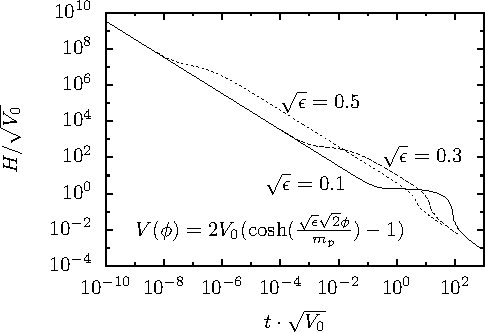
\includegraphics[width=\textwidth]{chapters/kinetic_dominance/figures/Hlam}
  \caption{As in Figure~\protect\ref{fig:figure_Hpol}, but for the hyperbolic cosine potential~\protect\eqref{eqn:coshpot}, which tends to an exponential potential for $\phi \to \pm\infty$. The scaling constant is now $\sqrt{V_0}$, and three values of $\sqrt{\epsilon}$ are considered. One can see clearly that the Universe emerges in a kinetically dominated state with $H=1/(3t)$. The Universe then enters a protracted power-law phase where $H = 1/(\epsilon t)$. The field $\phi$ oscillates about the base of the potential after the exit of the inflationary phase, causing wiggles in the later sections of the above plot.\label{fig:figure_Hlam}}
\end{figure}
%

%
\begin{figure}[tp]
  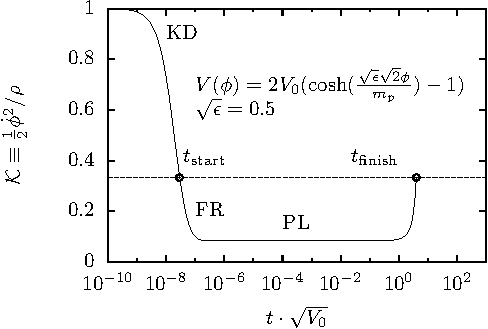
\includegraphics[width=\textwidth]{chapters/kinetic_dominance/figures/Klam}
  \caption{As in Figure~\protect\ref{fig:figure_Kpol}, but for the hyperbolic cosine inflaton potential with $\sqrt{\epsilon}=0.5$. The Universe emerges in a kinetically dominated (KD) phase before going through transitory fast-roll (FR). Instead of a slow-roll inflation, the Universe then settles into a power-law inflation (PL), characterized by $\Kfrac=\epsilon/3$. The Universe exits inflation at $t_\mathrm{finish}$, after which $\phi$ executes oscillations about the base of the potential. $\Kfrac$ therefore oscillates rapidly between $0$ and $1$, and the later $t>t_\mathrm{finish}$ section of this plot has been suppressed for clarity.\label{fig:figure_Klam}}
\end{figure}
%

We show the evolution of the Universe governed by the hyperbolic cosine inflaton potential~\eqref{eqn:coshpot} in Figures~\ref{fig:figure_Hlam}~\&~\ref{fig:figure_Klam}. The analysis is the same as that presented in Section~\ref{sec:section_polynomial_potentials}.  As in our previous example, the Universe emerges from the initial singularity in kinetic dominance, which then transitions through a brief period of fast-roll inflation into a generically long-lasting power-law inflation state until the exit is reached as $\phi\rightarrow0$, which corresponds to the minimum of the potential.  

\subsection{Another example of a finite solution $f(\psi)$}
The $f(\psi)$ described above in equation~\eqref{eqn:uf_power_law} is one of the simplest examples of a finite solution. As shown earlier, there is at most one such finite solution for any given potential. For concreteness we demonstrate another less trivial example in this section.

By reverse-engineering the master equation~\eqref{eqn:master_eq_f}, one can find a potential $V(\psi)$ for any specified $f(\psi)$. For example, if one chooses the oscillating solution (shown in Figure~\ref{fig:figure_uf}):
%
\begin{equation}
  f(\psi) = \log\left( \frac{1}{\sqrt{1-{[a+b\cos(2k\psi)]}^2}}\right),
  \label{eqn:uf_example}
\end{equation}
%
then this $f(\psi)$ is the finite solution of the potential defined by:
%
\begin{equation}
	V(\psi)
    =
    \left[ 1-{(a+b \cos2k\psi)}^2 \right]
    e^{2 a \psi +\frac{b}{k} \sin 2k\psi},
    \label{eqn:Vphi_uf_example}
\end{equation}
whose shape is detailed in Figure~\ref{fig:figure_ospot}.
%

To show explicitly that this is the only finite solution in this case, we consider a perturbed solution $y(\psi) = f(\psi)+\delta(\psi)$.  From the uniqueness theorem (Section~\ref{sec:uniqueness_theorem}) if $\delta$ is initially positive (negative), then it is positive (negative) for all $\psi$. From the master equation~\eqref{eqn:master_eq} one may show that the perturbed solution satisfies:
%
\begin{align}
  \frac{\d{}}{\d{\phi}}\delta 
  =& 
  \sqrt{1-e^{-2(f+\delta)}} -\sqrt{1-e^{-2f}}, 
  \label{eqn:perturb}
  \\
  &>
  \sqrt{1-e^{-2(\fm+\delta)}} -\sqrt{1-e^{-2\fm}}
\end{align}
%
where $\fm = \log(1/\sqrt{1-{(a-b)}^2})$. Substituting this in, one finds:
%
\begin{align}
  \frac{\d{}}{\d{\phi}}\delta 
  > 
  \sqrt{1-e^{-\delta}({1-{(a-b)}^2})} - \sqrt{1-({1-{(a-b)}^2})}
\end{align}
%
One can see that if $\delta>0$, then the right-hand side is strictly greater than some number greater than zero, hence $\delta$ grows without bound, and any solution greater than $f$ initially diverges. 

Working from equation~\eqref{eqn:perturb}, one also finds:
%
\begin{align}
  \frac{\d{}}{\d{\phi}}\delta 
  <&
  \sqrt{1-e^{-2(\fmn+\delta)}} -\sqrt{1-e^{-2\fmn}} 
  \nonumber
  \\
  &<
  \sqrt{1-e^{-\delta}({1-{(a+b)}^2})} - \sqrt{1-({1-{(a+b)}^2})}
\end{align}
%
One can see that if $\delta<0$, then the right-hand side is strictly less than some number less than zero, hence $\delta$ falls without bound, and any solution less than $f$ eventually becomes negative. 

Thus one finds that $f(\psi)$ is the only finite positive solution.  All other solutions either become negative or diverge.





%
\begin{figure}[tp]
  \centering
  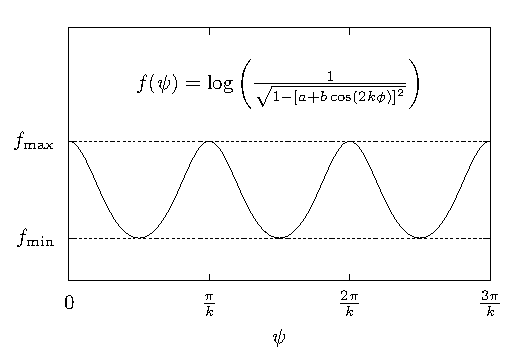
\includegraphics[width=\textwidth]{chapters/kinetic_dominance/figures/uf}
  \caption{An oscillating finite solution to the master equation~\protect\eqref{eqn:master_eq} with $V(\psi)$ defined as in equation~\protect\eqref{eqn:Vphi_uf_example} and demonstrated in Figure~\protect\ref{fig:figure_ospot}. If $a$ and $b$ are chosen such that $a>b>0$, $0<a+b<1$, $0<a-b<1$, then this represents a finite, positive solution.  From equation~\protect\eqref{eqn:uf_example} it is easy to see that $\fmn = \log\left(\frac{1}{\sqrt{1-{(a+b)}^2}}\right)$, $\fm=\log\left(\frac{1}{\sqrt{1-{(a-b)}^2}}\right)$.\label{fig:figure_uf}}
\end{figure}
%

%
\begin{figure}[tp]
  \centering
  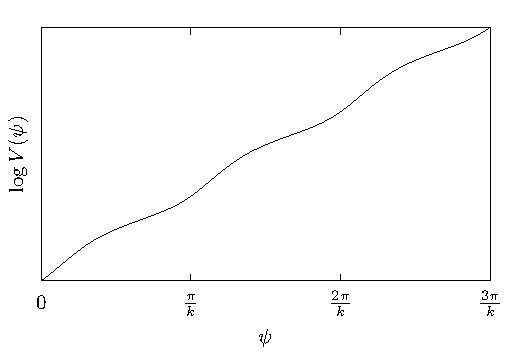
\includegraphics[width=\textwidth]{chapters/kinetic_dominance/figures/ospot}
  \caption{The master equation may be solved for the potential $V(\psi)$ if a form of $f(\psi)$ is chosen. For the choice of $f(\phi)$ detailed in equation (\protect\ref{eqn:uf_example}), the potential is solvable in closed form [equation \protect\ref{eqn:Vphi_uf_example}].\label{fig:figure_ospot}}
\end{figure}
%





\subsection{Power spectrum of the curvature perturbation}
\label{sec:powspec}

The most interesting aspect of kinetic dominance is seen when the power spectrum of scalar curvature perturbations is examined. Recent observations of CMB power spectra \citep{hinshaw_nine-year_2012,planck_collaboration_planck_2013} show an unexpected suppression at low multipoles. While these deviations are not large enough to cause us to discard the standard $\Lambda$ cold dark matter ($\Lambda$CDM) cosmology \citep{1998PhRvD..57.2207B,2000PhRvD..62l3513B,2004PhRvD..69f3516D}, there is still enough tension to be worthy of investigation.  As we show below, kinetic dominance predicts a generic cutoff in the curvature power spectrum at large spatial scales. This is precisely what is needed to suppress low multipole moments of the CMB power spectrum while retaining the quality of the fit at higher $\ell$ values.

Figure~\ref{fig:experimental_power_spectrum} has been taken from \citet{hlozek_atacama_2012} and shows the current status of the observational constraints on the late-time matter power spectrum, given by:
%
\begin{equation}
  P(k,z=0) = 2\pi^2 k \mathcal{P}_\mathcal{R}(k) G^2(z) T^2(k),
\end{equation}
%
where $G(z)$ gives the growth of matter perturbations, $T(k)$ is the matter transfer function and $\mathcal{P}_\mathcal{R}(k)$ is the primordial curvature perturbation power spectrum. This mapping enables one to combine constraints on the power spectrum from CMB and other probes at $z\approx 0$.




As shown by \citet{liddle_cosmological_2000}, the primordial curvature perturbation power spectrum $\mathcal{P}_{\mathcal{R}}(k)$ is given approximately by:
%
\begin{equation}
  \mathcal{P}_{\mathcal{R}}(k)
  =
  {\left(\frac{H^2}{2\pi\dot{\phi}}\right)}^2_{k=a H},
  \label{eqn:curvature_power_spectrum}
\end{equation}
%
where, as denoted, the right-hand side is evaluated when a given scale crosses the horizon. If one has numerically calculated $a(t)$, $H(t)$ and $\dot{\phi}(t)$, then plotting ${\left(H^2/ 2\pi\dot{\phi}\right)}^2$ against $aH$ will give the shape of the spectrum.

In order to perform predictive calculations, one must calibrate the $aH$ axis to an observable scale today. This is easy to do if one defines a comoving pivot scale $k_*$, which leaves the horizon (at a time $t_*$) when $N_*$ $e$-folds of inflation remain. In general, the relation between $k_*$ and $N_*$ depends on both the potential $V(\phi)$ and the details of cosmic reheating. For most reasonable models, $50<N_*<60$  for $k_*$ with a value of $0.05\:\mathrm{Mpc}^{-1}$ today \citep{planck_collaboration_planck_2013-1}. For this work, we will take $N_*=55$. 

Once a value for $N_*$ is chosen, one can determine numerically the time $t_*$ at which $N_*$ $e$-folds of inflation remain as well as $a_*\equiv a(t_*)$ and $H_*\equiv H(t_*)$. Since we know that the value of $aH$ at $t_*$ corresponds to a wave number today of $0.05\:\mathrm{Mpc}^{-1}$, we may calibrate the $aH$ axis of the plot of the power spectrum using:
%
\begin{equation}
  k_\mathrm{today} 
  = 
  \frac{aH}{a_*H_*}\times0.05\:\mathrm{Mpc}^{-1}.
\end{equation}
%
Calibrated plots of $\mathcal{P}_\mathcal{R}(k)$ are found in Figures~\ref{fig:figure_CSpol} and \nolinebreak\ref{fig:figure_CSlam}. 



The shape of the primordial power spectra obtained corresponds to that found in \citep{lasenby_closed_2003}. We see that, in general, $\mathcal{P}_\mathcal{R}(k)$ has less power at low and high $k$ values than would be expected from a canonical power-law primordial spectrum.  The low-$k$ cutoff is entirely generic and occurs as a result of the brief period of fast-roll prior to slow-roll or power-law inflation.  This effect has been discussed previously by Boyanovsky, de Vega and Sanchez (BVS) in \citep{boyanovsky_cmb_2006}. The fast-roll regime behaves like an attractor potential in the wave equations for the mode functions of curvature and tensor perturbations. This potential leads then to the suppression of the primordial power spectra at low $k$.  Hence, it might be able to account for the suppression of the quadrupole of the CMB in agreement with observational data, as discussed in \citep{boyanovsky_cmb_2006-1}.  The exact position of the low-$k$ cutoff is determined by the value of $\phip$, as it controls the total number of $e$-folds of inflation. This effect has also been discussed in the context of ``Open Inflation'' \citep{Yamauchi_strings_2011,Linde_open_1999,Linde_toy_1999}, and examined using WMAP data in \citet{Contaldi_suppress_2003}.

Further inspection shows $\mathcal{P}_\mathcal{R} \sim \log k$ after the low-$k$ cutoff. This is identical to the result found by \citet{lasenby_closed_2003} and in contrast with the standard power-spectrum parametrization which assumes a near-flat power-law scaling: $\log\mathcal{P}_\mathcal{R}\sim \log k$. 

 
It should be observed that we are using the approximation~\eqref{eqn:curvature_power_spectrum} outside the slow-roll regime for which it is valid; nonetheless we have performed full calculations that do not use the above approximation and which indicate that the resulting power spectrum is, in fact, a good representation of the true spectrum. These approximate spectra demonstrate the key generic aspects of the accurate calculation: both exhibit a low-$k$ cut off and that $\mathcal{P}_\mathcal{R}(k) \sim \log(k)$.  We shall follow this work with a second publication containing the full details and discussion of the accurate calculation. An alternative but related accurate calculation has been performed by \citep{Lello_tensor_2013}, which uses kinetic initial conditions to show that the suppression at low-$\ell$ is entirely generic. It should also be noted that methods which reconstruct the primordial power spectrum $\mathcal{P}_\mathcal{R}(k)$ \citep{vazquez_reconstruction,Hazra_reconstruction_2013} using data also show a dip at low $k$ values.

We demonstrate the suppression on large angular scales of the CMB and late-time matter power spectra qualitatively in Figure~\ref{fig:figure_Cl}.  In the standard six-parameter $\Lambda$CDM cosmology, the primordial power spectrum has a power-law form, parametrized by two variables $A_s$ and $n_\mathrm{s}$, such that:
%
\begin{equation}
  P_\mathcal{R}(k) = A_s{\left(\frac{k}{k_*}\right)}^{n_\mathrm{s}-1}
\end{equation}
%
Using the best-fit parameters from {\em Planck\/}+WP+highL+BAO \citep{planck_collaboration_planck_2013} yields the standard matter CMB power spectra (dashed lines), whereas the alternative power spectra (solid line) were generated using $\mathcal{P}_\mathcal{R}(k)$ from Figure~\ref{fig:figure_CSpol} (for $n=2$), for which the axes were rescaled to agree with the values of $A_s$ and $n_\mathrm{s}$ during the slow-roll phase. The resulting matter and CMB power spectra are seen to exhibit a suppression of power at low $k$ and $\ell$ values, with the rest of the spectra perfectly intact, as required by cosmological observations.  Further investigation is clearly required, but this analysis already demonstrates the utility of kinetic dominance.

%
\begin{figure}[tp]
  \centering
  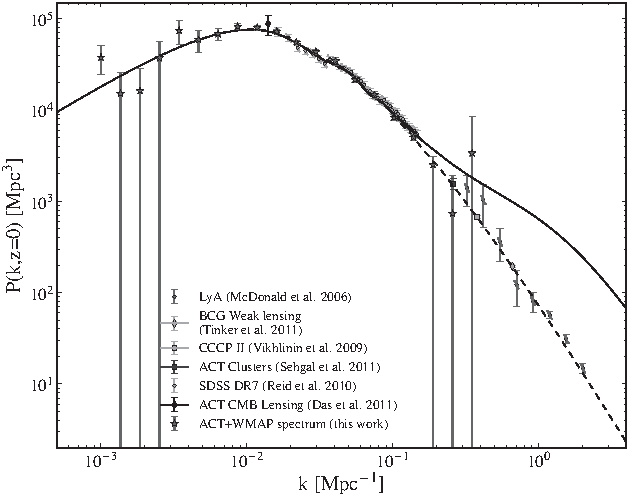
\includegraphics[width=\textwidth]{chapters/kinetic_dominance/figures/powerspec}
  \caption{Figure taken from \protect\citet{hlozek_atacama_2012} showing the current status of the observed late-time matter perturbation power spectrum. As one can see, the currently probed $k$ range is $10^{-3}<k<2\:\mathrm{Mpc}^{-1}$.\label{fig:experimental_power_spectrum}}
\end{figure}
%

%
\begin{figure}[tp]
  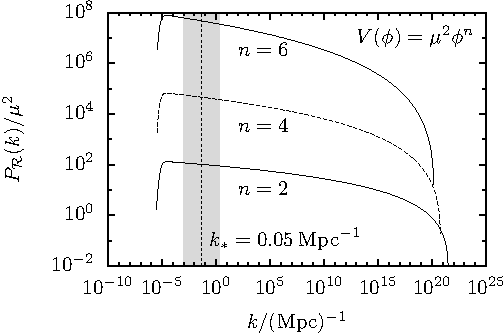
\includegraphics[width=\textwidth]{chapters/kinetic_dominance/figures/CSpol}
  \caption{The approximate power spectrum of the primordial curvature perturbations for polynomial potentials, calculated using equation~\protect\eqref{eqn:curvature_power_spectrum}. The units of the $k$ axis are determined by the requirement that there are $N_*=55$ $e$-folds remaining when the pivot scale $k_*=0.05\:\mathrm{Mpc}^{-1}$ exits the horizon $k=aH$. The magnitude of the power spectrum is determined by the scaling $\mu$ in the potential. The grey area indicates the angular scales that have been experimentally probed; see Figure~\protect\ref{fig:experimental_power_spectrum}.\label{fig:figure_CSpol}}
\end{figure}
%

%
\begin{figure}[tp]
  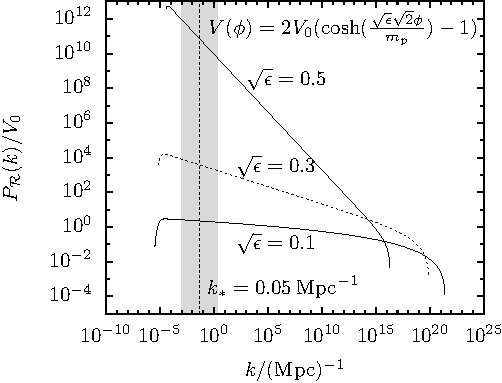
\includegraphics[width=\textwidth]{chapters/kinetic_dominance/figures/CSlam}
  \caption{As in Figure~\protect\ref{fig:figure_CSpol}, but for exponential potentials. The magnitude of the power spectrum now scales with $V_0$ rather than $\mu^2$.\label{fig:figure_CSlam}}
\end{figure}
%

%
\begin{figure}[tp]
  \centerline{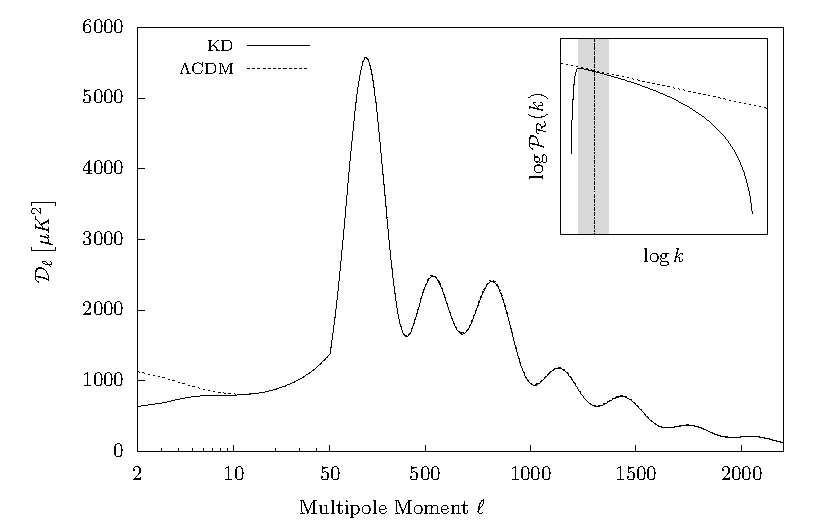
\includegraphics[width=\textwidth]{chapters/kinetic_dominance/figures/Cl}}
  \centerline{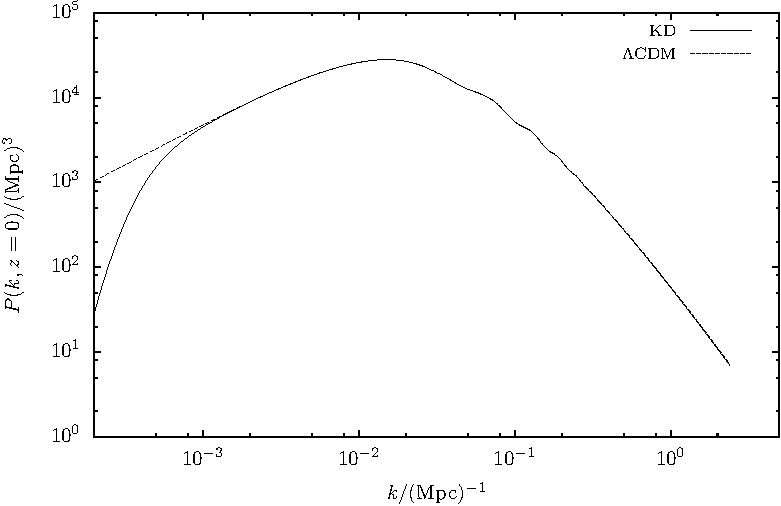
\includegraphics[width=\textwidth]{chapters/kinetic_dominance/figures/matter}}
  \caption{The CMB scalar power spectra (top) and the late-time matter power spectra (bottom), resulting from the curvature perturbation power spectra in the inset of the top figure. The solid line corresponds to a free inflaton with potential $V=\frac{1}{2}m^2\phi^2$ assuming kinetic initial conditions with $m=0.81\times10^{-5}\m$, $\phip = 21.8$, $N_*=42.5$. The dashed line corresponds to the best-fit standard $\Lambda$CDM model.  The presence of the cutoff in the curvature power spectrum for kinetic initial conditions causes a suppression of power on large angular scales in both the CMB and matter power spectra.\label{fig:figure_Cl}}
\end{figure}
%
The results of this section agree with the ``just enough inflation'' scenario introduced by \citet{Ramirez_excluded_2009,Ramirez_predictions_2012,Ramirez_low_2012}.  In their work they assume that there is some physical mechanism which would limit the potential from above such that $V(\phi)<M_\mathrm{GUT}^4$, and thus find that $V(\phi)\ll\dot{\phi}^2$ at early times. Our results therefore place their observations in a more generic setting.


\subsection{Comparison with equipartition initial conditions}
\label{sec:comparison}

An alternative method for setting the initial conditions for inflation models has been proposed by BVS in \citep{boyanovsky_cmb_2006}. Their work also shows that the low-multipole suppression of the scalar power spectrum is the result of a brief period of fast-roll inflation prior to the standard slow-roll regime. They arrange for such a fast-roll period by assuming ``equipartition initial conditions''. In this approach, the initial conditions are set at a time $t=\teq$, when there is approximate equipartition between the kinetic and potential energy of the inflaton:
%
\begin{equation}
  \frac{1}{2}\phideq \sim V(\phieq).
  \label{eqn:bvsbc}
\end{equation}
%
Almost by definition, the subsequent evolution will generically exhibit a (brief) period of fast-roll inflation, before entering a slow-roll phase (which is an attractor solution). BVS verified this generic behavior for a wide range of chaotic and new inflation potentials.

To address these issues further, we consider in more detail the main inflationary model used by BVS to illustrate their generic findings.  The model is spatially flat, and uses a ``new inflation'' potential:
%
\begin{equation}
  V(\phi) =V_0{\left(1-\mu\phi^2\right)}^2.
\end{equation}
%
The initial conditions are set by choosing $\phi(\teq)=\phieq=0$ with an equipartition of kinetic and potential energies so that $\dot{\phi}(\teq)=\phideq=\sqrt{2V_0}$.  Figure~\ref{fig:figure_BVS_initial_conditions} illustrates this diagrammatically.  The values of $V_0$ and $\mu$ are tuned so that the power spectrum has an appropriate index $n_s$ and the correct number of $e$-folds are generated.

%
\begin{figure}[tp]
  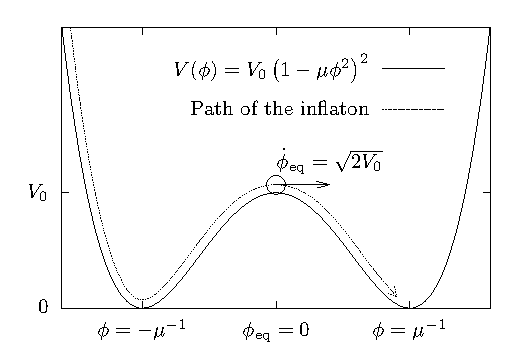
\includegraphics[width=\textwidth]{chapters/kinetic_dominance/figures/newpot}
  \caption{An illustration of the ``equipartition'' initial conditions imposed by \protect\citet{boyanovsky_cmb_2006}, for the new inflation potential $V_0{\left(1-\mu^2\phi^2\right)}^2$. The initial conditions are set at some time $\teq$ with values denoted by a subscript ``eq''. The field is set with $\phieq=0$ and a velocity $\phideq= \sqrt{2V_0}$ so that the energy is partitioned equally between kinetic and potential energy: $V(\phieq) = \frac{1}{2}\phideq$.\label{fig:figure_BVS_initial_conditions}}
\end{figure}
%

We now interpret this methodology using our formalism. Kinetic initial conditions will inevitably lead to a time $\teq$ when the equipartition condition~\eqref{eqn:bvsbc} is satisfied. Thus, rather than considering~\eqref{eqn:bvsbc} as a fundamental physical principle, it should be regarded as a natural consequence of kinetic initial conditions. Moreover, this is true independently of any tuning that we apply to $\mu$ or $V_0$ and indeed of the potential. Moreover, demanding that~\eqref{eqn:bvsbc} is satisfied at $\phi=0$ corresponds to choosing a specific value of $\phip$ such that the field arrives at $\phi=0$ with an equipartition of kinetic and potential energy (This is illustrated in Figure~\ref{fig:figure_BVS_initial_conditions}).  If, however, $\phip$ is required to lie within a certain range of values in order to produce an appropriate number of $e$-folds of inflation, then the choice $\phieq=0$ may be inconsistent with kinetic dominance. This can only be resolved if one is free to choose a general point $\phieq$ for the position of equipartition.  

\section{When is kinetic dominance not the case?}
\label{sec:When_is_kinetic_dominance_not_the_case?}
Having looked in detail at the consequences of kinetic dominance, we enumerate the instances in which it does not hold. If kinetic dominance is not the case, then we can conclude that either
%
\begin{enumerate}
    \item as one moves backward in time $\dot{\phi}\to 0$, and the inflaton tends to a constant value; or
    \item there is no epoch before which we can say $\dot{\phi}\ne 0$, and the inflaton continues to oscillate as one moves backward in time.
\end{enumerate}
%
We shall examine each of these cases in turn.

\subsection{Resting inflaton: $\dot{\phi}\to 0$}


\subsubsection{No auxiliary fluids: eternal de Sitter}
We shall begin by considering the case with no auxiliary fluids, for which the Friedmann~\eqref{eqn:Friedmann_mod} and Klein-Gordon~\eqref{eqn:Klein_Gordon_mod} equations take the form:
%
\begin{align}
  H^2 
  &=
  \frac{1}{3\m^2}\left(\tfrac{1}{2}\dot{\phi}^2 + V(\phi) \right)
  \label{eqn:Friedmann_dotphi_to_zero_no_fluid} 
  \\
  0
  &=
  \ddot{\phi} +3\dot{\phi}H + V^\prime(\phi).
  \label{eqn:Klein_Gordon_dotphi_to_zero_no_fluid}
\end{align}
%
If $\dot{\phi}\to 0$ as one moves backward in time, then the inflaton $\phi$ and field $V(\phi)$ tend to constant values $\phiz$ and $V(\phiz)\equiv V_0$. By examining the first of the above equations, one can see that $H$ tends to a constant value:
%
\begin{equation}
  H\to H_0 \equiv \sqrt{\frac{V_0}{3\m^2}}.
\end{equation}
%
Thus, such a universe exhibits an eternal de Sitter phase (edS) as $t\to-\infty$.

By examining the Klein-Gordon equation~\eqref{eqn:Klein_Gordon_dotphi_to_zero_no_fluid}, one can see that the only nonzero term remaining is $\frac{\d{}}{\d{\phi}}V(\phi)$. From this one can conclude that the inflaton must come to rest on an extremum of the potential. It is straightforward to show that the dynamical equations then have the following asymptotic solution as $t \to -\infty$:
%
\begin{align}
  \phi(t)
  &=
  \phiz \pm A \exp(\alpha t),\\
  H(t)
  &=
  \sqrt{\frac{V(\phiz)}{3\m^2}} \equiv H_0,\\
  a(t)
  &=
  B e^{H_0t},
\end{align}
%
where $A$ and $B$  are arbitrary constants, and $\alpha$ is a real, positive solution to the quadratic equation:
% 
%
\begin{equation}
  \alpha^2 + 3H_0\alpha + \left.
  \frac{{d^2}V}{{d}\phi^2}\right|_{\phi=\phiz}=0.
\end{equation}
%
This solution is discussed in more detail by \citet{destri_preinflationary_2010}. An example of this is ``Hilltop inflation'' \citep{linde_1982,albrecht_1982}. 

It should be noted that these solutions are not generic, as these solutions are rolling away from a position of unstable equilibrium: going backward in time, any small perturbation causes the inflaton to overshoot the extremum and move on to a kinetically dominated phase.

One can demonstrate the above statement formally by considering equations~\eqref{eqn:Klein_Gordon_dotphi_to_zero_no_fluid} and~\eqref{eqn:Friedmann_dotphi_to_zero_no_fluid} in the Hamilton-Jacobi representation:
%
\begin{align}
  {\left(\frac{\d{H}}{\d{\phi}}\right)}^2
  &=
  \frac{3H^2}{2\m^2} - \frac{V(\phi)}{2\m^4}
  \\
  \frac{\d{H}}{\d{\phi}}
  &=
  -\frac{\dot{\phi}}{2\m^2}.
\end{align}
%
The Hamilton-Jacobi representation is valid in the periods in which $\phi(t)$ is monotonic; i.e. $\dot{\phi}$ does not change sign. If one assumes that $\dot{\phi}>0$, then the first of the above equations reads:
%
\begin{equation}
  \frac{\d{H}}{\d{\phi}} 
  = 
  -\sqrt{\frac{3H^2}{2\m^2} - \frac{V(\phi)}{2\m^4}}.
  \label{eqn:Hamilton_Jacobi_H}
\end{equation}
%
Solutions to this equation are plotted in Figure~\ref{fig:figure_edS}, which demonstrates the following facts: 
%
\begin{itemize}
  \item There is a region in which solutions cannot exist, since by the Friedmann equation~\eqref{eqn:Friedmann_dotphi_to_zero_no_fluid} we find that $H>\sqrt{V(\phi)/3\m^2}$.
  \item  By equation~\eqref{eqn:Hamilton_Jacobi_H} that solutions meet this region with zero gradient.
  \item Outside of this region, the right-hand side of equation~\eqref{eqn:Hamilton_Jacobi_H} is Lipschitz continuous (see Section~\ref{sec:uniqueness_theorem}, or \citet{agarwal_1993}), hence solutions do not cross over in the white region of the graph.
\end{itemize}
% 

Consider the eternal de Sitter solution $\HedS(\phi)$, plotted as the right-hand half of the dotted line in Figure~\ref{fig:figure_edS}.  This solution has the property that as $\phi\to\phiz$, $\dot{\phi}\propto\frac{\d{H}}{\d{\phi}}\to0$. Consider also a solution $\Hh$ which at some value $\phi_1$ is greater than the edS solution, $\Hh(\phi_1) \ge \HedS(\phi_1)$. By uniqueness, this will remain greater than $\HedS$ within the white region of the graph. Both $\HedS$ and $\Hh$ satisfy equation~\eqref{eqn:Hamilton_Jacobi_H}.  Taking the difference of these two equations and integrating from $\phi_1$ to $\phiz$ shows:
%
\begin{align}
  &\Hh(\phiz)-\HedS(\phiz)= \nonumber\\
  &\Hh(\phi_1)-\HedS(\phi_1) \nonumber\\
  & + \int_{\phiz}^{\phi_1} 
  \sqrt{\frac{3\Hh^2}{2\m^2} - 
  \frac{V(\phi)}{2\m^4}}-\sqrt{\frac{3\HedS^2}{2\m^2} - 
  \frac{V(\phi)}{2\m^4}}\:d\phi \nonumber \\
  &>\Hh(\phi_1)-\HedS(\phi_1)>0 \nonumber
\end{align}
%
We thus find ${d\Hh}/{d\phi}\ne0$ at $\phi=\phiz$, and thus does not represent an eternal de Sitter phase. A similar argument holds for solutions $\Hl(\phi)$ which start out less than $\HedS$, only these must collide with the dark region. Upon this collision, $\dot{\phi}$ changes sign, causing the diagram to reflect about the $\phi=0$ axis.

Figure~\ref{fig:figure_edS} reveals an interesting second eternal de Sitter solution. The right-hand half of the dashed line indicates the previously discussed phase: a universe which emerges at $t=-\infty$ in an inflating state with the inflaton slowly rolling off an extremum in the potential, exiting the inflationary phase when the inflaton oscillates about the bottom of the potential.  The left-hand half of the dashed line indicates a universe which emerges at $t=0$ in a kinetically dominated phase before the inflaton rests on top of the extremum, settling into an eternal de Sitter phase as $t\to\infty$.

%
\begin{figure}[tp]
  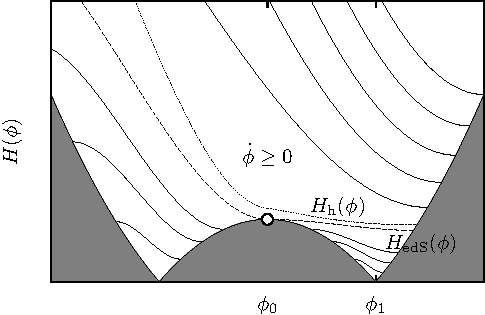
\includegraphics[width=\textwidth]{chapters/kinetic_dominance/figures/edS}
  \caption{Schematic of the Hubble parameter against $\phi$ in the Hamilton-Jacobi representation. The potential $V(\phi)$ is the same potential as in Figure~\protect\ref{fig:figure_BVS_initial_conditions}. The solid curves represent the portions of the solutions to~\protect\eqref{eqn:Hamilton_Jacobi_H} with $\dot{\phi}\ge0$. The shaded region is defined by $H<\sqrt{V/3\m^2}$. Solutions meet the shaded region with zero gradient. Solutions within the white region are unique: they do not cross over. The right-hand side of the dashed curve represents a universe entering at  $\phi=\phiz$, ($t=-\infty$) in an eternal de Sitter phase. The left-hand side of the dashed curve indicates a universe entering in a kinetically dominated phase before settling into a de Sitter phase at $t=+\infty$.\label{fig:figure_edS}}
\end{figure}
%

\subsubsection{Auxiliary fluids}
The presence of an auxiliary fluid makes it slightly easier to engineer a solution in which $\dot\phi\to0$, as one does not require that the inflaton comes to rest on an extremum of the potential.

In the limit that $a\to 0$, the $\rho_i$ with the largest $w_i$ dominates over all of the others. The relevant equations are therefore the Friedmann~\eqref{eqn:Friedmann_mod} and Klein-Gordon~\eqref{eqn:Klein_Gordon_mod} equations, with a single fluid $\rho_w$:
%
\begin{align}
  H^2
  &=
  \frac{1}{3\m^2}\left(\tfrac{1}{2}\dot{\phi}^2
  + V(\phi)
  + \rho_w \right),
  \label{eqn:Friedmann_dotphi_to_zero} \\
  0
  &=
  \ddot{\phi} +3\dot{\phi}H + V^\prime(\phi).
  \label{eqn:Klein_Gordon_dotphi_to_zero}
\end{align}
%
In the first of these, if $\phi\to\phiz$, then as $a\to0$ on the right-hand side one only need worry about $\rho_w$. Since $H=\frac{\d{}}{\d{t}}\log a$, and $\rho_w\propto a^{-3(1+w)}$, one finds:
%
\begin{align}
  \int\frac{\d{\log a}}{\sqrt{\rho_w}}
  &=
  \int\frac{t}{\sqrt3\m}
  \\
  \Rightarrow \qquad \rho_w
  &=
  \frac{4\m^2}{3{(1+w)}^2} \frac{1}{t^2}.
  \label{eqn:rho_dotphi_to_zero}
\end{align}
%
We may then use the above equation along with~\eqref{eqn:Friedmann_dotphi_to_zero} to show that:
%
\begin{equation}
  H = \frac{2}{3(1+w) t}
  \quad
  \Rightarrow \quad a\propto t^{2/3(1+w)}.
  \label{eqn:H_dotphi_to_zero}
\end{equation}
%
We can now solve~\eqref{eqn:Klein_Gordon_dotphi_to_zero} for $\phi(t)$.  As $\phi\to\phiz$, we may assume the potential term tends to a constant value $\prm{V_0}$. Selecting the solution which tends to a constant, one finds:
%
\begin{equation}
  \phi(t) = \phiz -\frac{\prm{V_0}(w+1)}{2(w+3)}t^2.
\end{equation}
%
This constitutes a solution which is present for any potential with auxiliary fluids. In general one can find a specific solution with $\phi\to\phiz$ for any given $\phiz$. However, for any small perturbation from this solution, one arrives back at kinetic dominance. The kinetically dominated solutions are generic. 












\subsection{Pathological oscillations: $\dot{\phi}=0$}
We now turn to the case where there is no epoch prior to which $\phi$ is monotonic. The inflaton continues to oscillate endlessly as $a\to0$. 

It is easy to engineer potentials that lead to this behavior. In the case with no auxiliary fields, the limiting forms of $\dot{\phi}(t)$ and $\phi(t)$ are given by equations~\eqref{eqn:dotphi_of_t_flat} and~\eqref{eqn:phi_of_t_flat}. We may solve these to find the relationship between $\dot{\phi}$ and $\phi$:
%
\begin{equation}
  \dot{\phi}^2 = \exp\left(\frac{\sqrt{6}}{\m} |\phi-\phip|\right).
\end{equation}
%
If one chooses a potential that grows faster than the right-hand side of this equation, then the universe cannot be kinetically dominated.  We are thus forced to the conclusion that in such a universe either $\dot{\phi}\to 0$ or there is no epoch before which $\dot{\phi}\ne 0$.  Typically, if one examines the numerical solutions of such equations, one sees that the inflaton oscillates at a faster and faster rate, with greater and greater amplitude until the numerical limit of the solver is reached.

These solutions are therefore somewhat pathological, though for the cases where they occur, kinetic dominance is not the generic solution.









\section{Conclusions}
\label{sec:Conclusions}

We have shown that, if quantum gravitational effects are ignored, the coupled evolution equations for the inflaton field $\phi(t)$ and the Hubble parameter $H(t)$ in generic homogeneous and isotropic single-field inflation models imply that a universe beginning with a steadily moving inflaton ($|\dot{\phi}| > \vellim > 0$ as $a\to 0$, for some positive constant $\vellim$) generically emerges from an initial singularity in a noninflating, kinetically dominated state ($\dot{\phi}^2 \gg V(\phi)$).  In this kinetic-dominated regime, one obtains simple analytical solutions for $\phi(t)$ and $H(t)$, which are independent of the form of the inflaton potential $V(\phi)$ and of the presence of auxiliary fluids such as matter, radiation, dark energy or spatial curvature. These solutions provide a simple means of setting the initial conditions for such inflation models, from which numerical integration of the evolution equations may proceed.

For illustration, we applied this ``kinetic'' procedure for setting initial conditions to a spatially flat polynomial and exponential inflation models.  By making an appropriate choice of the time $\ti$ at which the initial conditions are set, and the single free parameter $\phip$ in the analytic kinetic-dominated solution, all models produce an amount of inflation compatible with observations.  The background evolution in each case displays a generic behavior.  Following a noninflating period of kinetic dominance, $H(t)$, $\phi(t)$ and their time derivatives continue to decrease until one obtains approximate equipartition $\dot{\phi}^2 \sim V(\phi)$ between the kinetic and potential energies of the inflaton. This marks the onset of a (typically brief) period of fast-roll inflation, which turns into a slow-roll [$\dot{\phi}^2 \ll V(\phi)$] or power-law inflation phase.  At the end of the slow-roll phase, the inflation quickly moves towards a minimum of the potential, about which it executes a decaying oscillation.

We calculated the approximate spectrum of scalar perturbations for the polynomial and exponential models and find, in both cases, that it contains less power at low- and high-$k$ values than would be expected from a power-law behaviour. The low-$k$ effect is a generic consequence of the kinetic initial conditions, for any consistent inflaton potential or spatial curvature, resulting in particular from the brief period of fast-roll inflation that they imply.  The damping of power on large scales may provide an explanation for the low-$\ell$ falloff in the matter and CMB power spectra seen in recent cosmological observations.

We also compared our kinetic initial conditions with an alternative proposal by \citet{boyanovsky_cmb_2006} that inflationary initial conditions should be set by assuming approximate equipartition between the kinetic and potential energy of the inflaton.  In the context of kinetic initial conditions, approximate equipartition is not a fundamental physical principle, but merely an inevitable consequence.  Moreover, by considering a particular model used by BVS, we demonstrate that assigning equipartition initial conditions with an arbitrary initial value for the inflaton field can lead to inconsistency with kinetic initial conditions.

Finally we enumerated the universes which do not have a steadily moving inflaton, and have shown that these are special cases, distinct from the generic kinetically dominated case.

\section*{Acknowledgements}
We thank Norma Sanchez for providing useful comments on a very early version of this paper originally drafted in June 2009. We also thank the two anonymous referees for numerous useful comments. S.D.B.\ thanks the Isaac Newton Trust and the Sunburst Fund for their support. W.J.H.  thanks STFC for their support




\begin{subappendices}
  \section{Uniqueness theorem}
\label{sec:uniqueness_theorem}
We shall now prove that the solutions to the initial value problem of the master equation~\eqref{eqn:master_eq}:
%
\begin{align}
  \frac{\d{y}}{\d{\psi}}
  &=
  \sqrt{1-e^{-2y}} - \frac{\d{}}{\d{\psi}}\log \sqrt V,
  \label{eqn:IVP1}
  \\
  y(\psiz)
  &=
  y_0>0
  \label{eqn:IVP2},
\end{align}
%
are unique within any finite interval \(\psi\in[\psiz,\psi_1]\); i.e, if two positive solutions intersect at a point, then they intersect
everywhere.

We begin by putting a lower bound on \(y\) in the interval \([\psiz,\psi_1]\): From assumption~\eqref{eqn:conditions}, we know \(\dot{\phi}^2>\vellim^2>0\). If we unpack the definition of \(y\) using equations~\eqref{eqn:y_def},~\eqref{eqn:Ntrans},~\eqref{eqn:tau_def} and~\eqref{eqn:Friedmann_c}, one finds:
%
\begin{equation}
  y 
  = 
  \frac{1}{2}\log
  \left(\frac{\frac{1}{2}\dot{\phi}^2 + V(\phi)}{V(\phi)}\right) 
  > 
  \frac{\vellim^2}{4\Vm},
\end{equation}
%
where \(\Vm\) is the maximal value of \(V(\psi)\) in the interval \([\psiz,\psi_1]\). With this in hand we may prove the uniqueness of solutions of the initial value problem~\eqref{eqn:IVP1},~\eqref{eqn:IVP2} using standard techniques. For a good reference of such techniques the reader should consult the text by \citet{agarwal_1993}. In this case, we shall prove it using {\em Peano iteration}.


If one assumes that \(y(\psi)\) and \(z(\psi)\) are two distinct solutions, then their difference satisfies:
%
\begin{equation}
  \frac{\d{}}{\d{\psi}}(y-z)
  =
  \sqrt{1-e^{-2y}} - \sqrt{1-e^{-2z}}.
  \label{eqn:master_diff}
\end{equation}
%
If in addition one assumes they meet at a common point \(\psi_0\), so that \(y(\psi_0)=z(\psi_0)\), then integrating away from this position yields:
%
\begin{align}
  \abs{y(\psi)-z(\psi)}
  &=
  \abs{\int_{\psi_0}^\psi \sqrt{1-e^{-2y}}
  - \sqrt{1-e^{-2z}}\:\:d\psi}
  \nonumber\\
  &
  \le \int_{\psi_0}^\psi \abs{\sqrt{1-e^{-2y}}
  - \sqrt{1-e^{-2z}}}d\psi.
  \label{eqn:ineq_1}
\end{align}
%
A generic property of the function \(f(y)=\sqrt{1-e^{-2y}}\) is that in the interval \(\left[\phantom(\frac{\vellim^2}{4\Vm},\infty\right)\phantom]\) it is {\em Lipschitz continuous\/}:
%
\begin{equation}
  \abs{\sqrt{1-e^{-2y}} - \sqrt{1-e^{-2z}}} \le L\abs{y-z},
  \label{eqn:Lipschitz}
\end{equation}
%
where \(L\) is the {\em Lipschitz constant}, taking the value:
%
\begin{equation}
  L
  = 
  \frac{\exp{\left(-\frac{\vellim^2}{2\Vm}\right)}}
  {\sqrt{1-\exp{\left(-\frac{\vellim^2}{2\Vm}\right)}}} 
  > 0.
\end{equation}
%                                              
Applying Lipschitz continuity~\eqref{eqn:Lipschitz} to the inequality in~\eqref{eqn:ineq_1} gives:
%
\begin{equation}
  \abs{y(\psi)-z(\psi)} 
  \le
  L\int_{\psi_0}^\psi\abs{y(\psi)-z(\psi)}\d{\psi}.
  \label{eqn:ineq_2}
\end{equation}
%
Further, if the maximum value of the difference of \(|y-z|\) between \(\psi_0\) and \(\psi\) is \(\Delta\), then the above implies:
%
\begin{equation}
  \abs{y(\psi)-z(\psi)} 
  \le
  L\Delta\abs{\int_{\psi_0}^\psi \d{\psi}}= 
  L\Delta\abs{\psi-\psi_0}.
\end{equation}
%
Applying this inequality back into~\eqref{eqn:ineq_2} shows:
%
\begin{equation}
  \abs{y(\psi)-z(\psi)} 
  \le
  L^2\Delta\int_{\psi_0}^\psi\abs{\psi-\psi_0}\d{\psi} =
  L^2\Delta\frac{\abs{\psi-\psi_0}^2}{2!}.
\end{equation}
%
Applying this back into~\eqref{eqn:ineq_2} yields:
%
\begin{equation}
  \abs{y(\psi)-z(\psi)} 
  \le
  L^3\Delta\frac{\abs{\psi-\psi_0}^3}{3!},
\end{equation}
%
and by induction on \(n\in\mathbb{N}\) we find that:
%
\begin{equation}
  \abs{y(\psi)-z(\psi)} 
  \le
  L^n\Delta\frac{\abs{\psi-\psi_0}^n}{n!}.
\end{equation}
%
As \(n\to\infty\) the term on the right-hand side drops to \(0\), and therefore \(|y(\psi)-z(\psi)|=0\). Thus, if \(y\) and \(z\) are equal at some point \(\psi_0\), then they are equal at all points \(\psi\) within any finite interval \([\psiz,\psi_1]\). Two separate solutions cannot ``cross over'', and if one positive solution \(f\) is initially less than a second solution \(h\) at \(\psiz\), \(f(\psiz)<h(\psiz)\), then \(f(\psi_1)<h(\psi_1)\) for any finite \(\psi_1\).  



\end{subappendices}

